\chapter{Methodology: From Pose Estimation to Decision}
\label{cap:metodologia}

This chapter sets out the methodology developed for the fall detection system, following the path that leads from the acquired frame to the generation of the alarm. As discussed in Chapter \ref{cap:stato_arte}, the decision is not taken on a single image, but on a sequence of consecutive observations.

The video enters the first stage of the pipeline, where the person's pose is estimated by means of MediaPipe Pose. The images are never passed to the classifier directly: from each frame the body landmarks are extracted, and from these the geometric and temporal quantities are computed. The model therefore works on a numerical representation of the movement, and not on the pixels of the image.

\section{Overview of the pipeline}
\label{sec:impostazione}

Figure \ref{fig:pipeline} summarises the complete pipeline.

\begin{figure}[htbp]
\centering
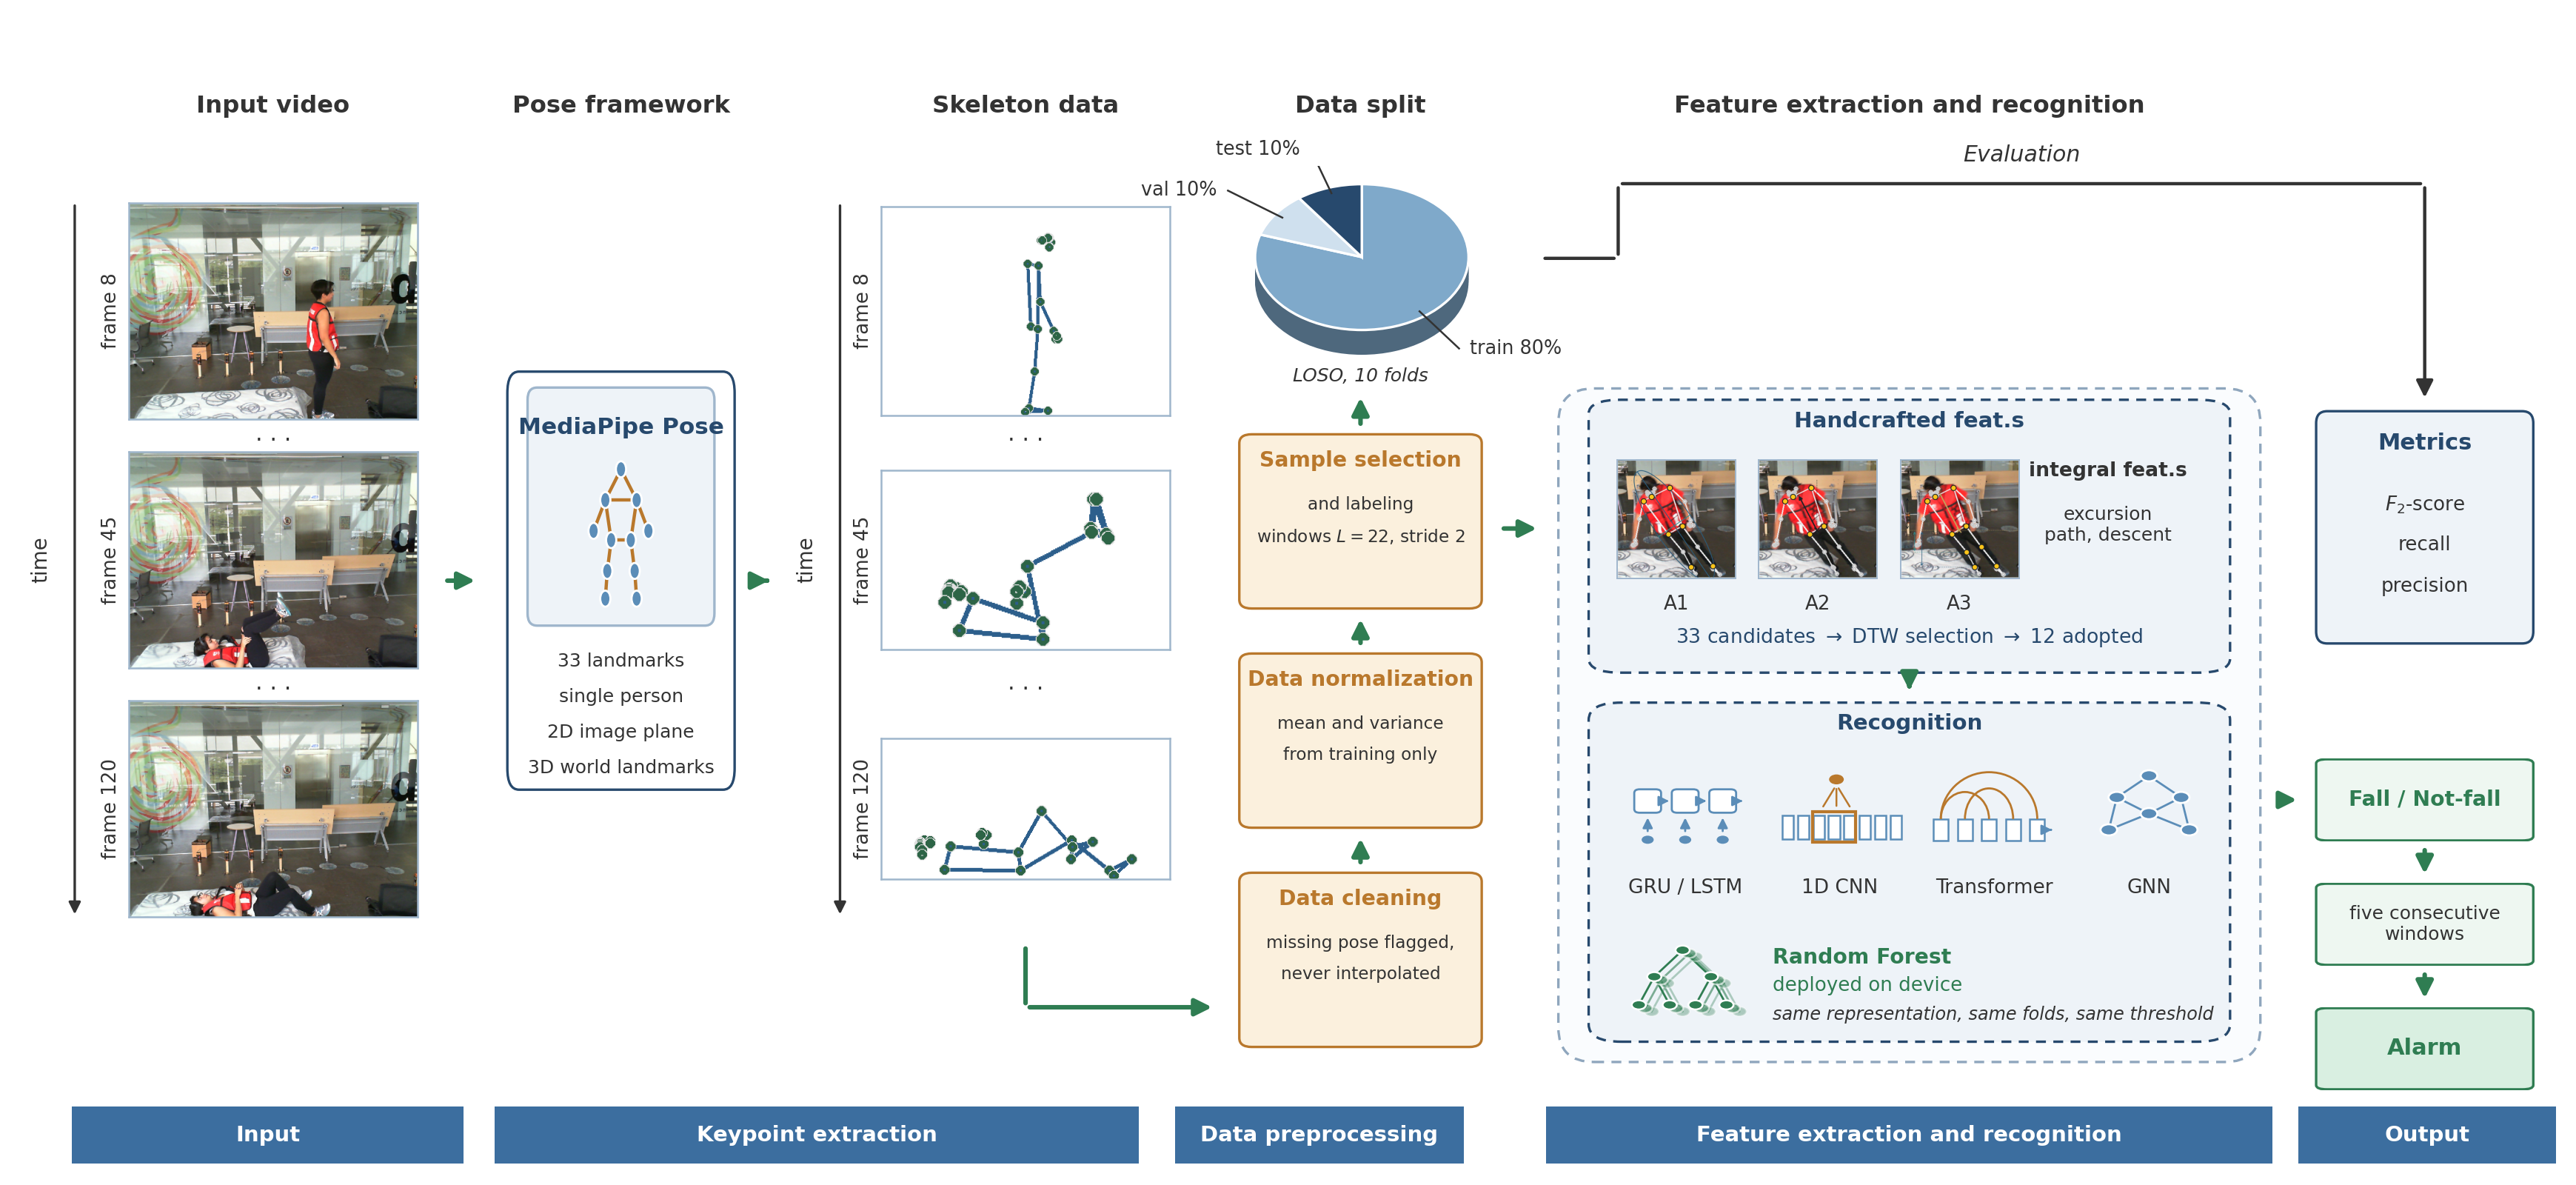
\includegraphics[width=\textwidth]{figure/fig_pipeline_en.png}
\caption{General scheme of the pipeline, from the RGB frame to the generation of the alarm event.}
\label{fig:pipeline}
\end{figure}

Every RGB frame is first turned into a skeletal pose. From the landmarks, 23 geometric and kinematic quantities are derived, to which are added nine quantities computed over longer time intervals and one measure of the position of the hips relative to the floor. This yields 33 candidate features. The set is subsequently reduced by a selection procedure based on \emph{Dynamic Time Warping}, which brings it down to 12 features. These are organised into temporal windows of 22 samples and used as the input of the classifiers.

Six architectures are compared in this work: Random Forest, LSTM, GRU, 1D CNN, Transformer and a graph network. The comparison keeps the input representation and the evaluation protocol unchanged as far as possible, so that what is measured is the contribution of the architecture. For each window the classifier produces a score associated with the presence of a fall. The decisions on the individual windows are finally aggregated over time to obtain the alarm events used during continuous operation. Table~\ref{tab:pipeline_1} summarises the main stages and shows how the information is progressively transformed.

\begin{table}[htbp]
\centering
\caption{Main stages of the pipeline, with their input and output.}
\label{tab:pipeline_1}
\resizebox{\textwidth}{!}{
\begin{tabular}{lllc}
\toprule
\textbf{Stage} & \textbf{Input} & \textbf{Output} & \textbf{Section} \\
\midrule
Pose estimation & RGB frame & 33 landmarks & \ref{sec:pose} \\
Geometric representations & landmarks & 23 quantities & \ref{sec:rappresentazioni} \\
Integral quantities & quantities & $+9$ & \ref{sec:integrali} \\
Height above the floor & quantities & $+1$ & \ref{sec:pavimento} \\
DTW selection & 33 candidates & 12 features & \ref{sec:dtw} \\
Temporal windows & feature sequence & $L=22$, stride 2 & \ref{sec:finestre} \\
Task and labels & windows & three training formulations & \ref{sec:compito} \\
Classifier & $22\times12$ window & score in $[0,1]$ & \ref{sec:classificatori} \\
Aggregation & scores & windows above threshold & \ref{sec:allarme} \\
Alarm event & windows above threshold & a single alert & \ref{sec:allarme} \\
\bottomrule
\end{tabular}
}
\end{table}

The protocol by which the models are evaluated --- LOSO partitioning, normalisation, metrics and decision threshold --- is described instead in Chapter~\ref{cap:sperimentale}.
\section{Experimental data and preprocessing}
\label{sec:dati}

The dataset used to develop the system is UP-Fall. Ten of the seventeen available subjects were considered, together with both views provided by the archive: one lateral, placed approximately at chest height, and one raised frontal. For the ten subjects, all \textbf{220 recordings} available were used, 110 for each camera. Of these, 100 contain falls and 120 ordinary activities of daily living (ADL), for a total of 116.362 frames. No recording was excluded.

UP-Fall does not distribute video files, but sequences of PNG images organised into folders, one per recording. The name of each file carries the timestamp of the instant of acquisition. For every sample, the information concerning subject, camera, recording and label is retained as well. Table~\ref{tab:dati} summarises the data used in the experiments and the main choices adopted for preprocessing.

\begin{table}[htbp]
\centering
\caption{Data used and main preprocessing operations.}
\label{tab:dati}
\begin{tabularx}{\textwidth}{@{}lX@{}}
\toprule
\textbf{Item} & \textbf{Configuration adopted} \\
\midrule
Dataset & UP-Fall \\
Subjects & 10 of the 17 available \\
Views & both cameras \\
Recordings & 220: 100 falls and 120 ADL \\
Frames & 116.362 \\
Recordings excluded & none \\
Declared frame rate & 18 fps \\
Measured frame rate & median 18,09 fps; 14,43--19,63 fps \\
Interpolation & none \\
Subsampling & one frame in two within the windows \\
Missing pose & the temporal sequence is broken \\
Normalisation & estimated within each fold \\
Feature selection & DTW applied once over the whole dataset \\
\bottomrule
\end{tabularx}
\end{table}

\subsection{Temporal cadence}
\label{sec:cadenza}

UP-Fall is declared at 18~fps \cite{MV}, but the timestamps carried by the file names allow the actual cadence to be measured directly. The median frequency is $18{,}09$~fps and ranges between $14{,}43$ and $19{,}63$~fps. In 70 of the 220 recordings the departure from the nominal value exceeds 5\%. The ten recordings furthest from that value all belong to the same individual.

The frequency is not constant within a single recording either. The interval between two consecutive frames has a median of $49{,}6$~ms, a ninth decile of $70{,}2$~ms and a ninety-ninth percentile of $159{,}8$~ms. For the quantities that depend on time, the actual interval $\Delta t_i=t_i-t_{i-1}$ is therefore used, instead of assuming a constant duration of $1/18$~s. This choice matters in the LOSO protocol as well: were the cadence taken as constant, the error on the kinematic quantities would differ from subject to subject and could therefore affect an entire fold.

The coordinates are not resampled onto a uniform time grid, so that no pose is ever created at an instant that was not directly observed. A subsampling is nevertheless applied when the windows are built, taking one frame in two, so that the nominal frequency supplied to the classifier drops from 18 to about 9 samples per second. Resampling to a common length is instead used during the DTW selection described in Section~\ref{sec:dtw}, where the curves are brought to 200 samples before being compared. That operation concerns the analysis of the features and does not alter the data supplied to the classifier.

\subsection{Frame-level labels}

The label of every frame is derived from the suffix \texttt{-0}, \texttt{-1} or \texttt{-2} carried by the name of the PNG file. The three labels denote, respectively, ordinary activity or the phase preceding the fall, the fall transition, and the post-fall state. Where the suffix is absent, the category of the folder is used instead. That decision is not harmless: inside a folder of falls, a frame without a suffix would be labelled as a fall even though the person is still standing. For this reason the program counts the cases in which it had to fall back on the default value and reports them. The resulting distribution is given in Table~\ref{tab:etichette}.

\begin{table}[ht]
\centering
\caption{Distribution of the frame-level labels over the 220 recordings used.}
\resizebox{\textwidth}{!}{
\begin{tabular}{llrr}
\toprule
\textbf{Label} & \textbf{Phase} & \textbf{Frames} & \textbf{Share} \\
\midrule
$0$ & ordinary activity, or the phase preceding the fall & 100.296 & 86,2\% \\
$1$ & fall transition & 5.542 & 4,8\% \\
$2$ & post-fall state & 10.524 & 9,0\% \\
\midrule
\multicolumn{2}{l}{\emph{total}} & 116.362 & 100\% \\
\multicolumn{2}{l}{\emph{with a valid pose}} & 111.570 & 95,9\% \\
\bottomrule
\end{tabular}
}
\label{tab:etichette}
\end{table}

The transition accounts for less than 5\% of the frames available, whereas the post-fall state is almost twice as frequent. This distribution is therefore strongly imbalanced, and it is taken up again both in the definition of the task and in the choice of the evaluation metrics.

Two kinds of interruption are distinguished. When the time interval between two consecutive images is longer than expected, no intermediate frames are reconstructed and the time that actually elapsed is retained. When, by contrast, the estimator returns no valid pose, the sequence is broken and the state used by the temporal features is reset. A window can therefore never span a loss of pose.

A valid pose is available in 95,9\% of the frames. That figure only indicates that the estimator returned a skeletal configuration; it does not measure the quality of the landmarks, which is examined in Section~\ref{sec:posa-mancante}.

The normalisation used by the classifiers is estimated within each fold, on the training data alone. Feature selection by DTW was instead carried out once over the whole dataset, before the LOSO validation, so that the test subject contributes indirectly to the choice of the features. This form of \emph{data leakage} is declared here and measured quantitatively in Section~\ref{sec:misura_leakage} of Chapter~\ref{cap:sperimentale}.

\section{Pose estimation}
\label{sec:pose}

RGB images are the initial data of the pipeline, but they are not used directly by the classifier. Each frame is first turned into a representation of the person's pose by means of a limited set of anatomical points, the \emph{landmarks}.
This transformation reduces the information available to what is essential in order to describe the configuration and the movement of the body. The system thus passes from a dense representation, made of pixels, to a sparse one composed of a few dozen coordinates.
There are two main advantages:
\begin{itemize}
    \item \textbf{reduction of dimensionality}: the system does not have to process hundreds of thousands of pixels directly, but only a limited number of coordinates;
    \item \textbf{interpretability}: each landmark represents a precise part of the body, which allows us to build quantities whose meaning is tied to the geometry and the movement of the person.
\end{itemize}

\subsection{Comparison between estimators}

Three pose estimators were considered over the course of the development; their differences are reported in Table \ref{tab:pose}.

\begin{table}[htbp]
\caption{Main characteristics of the pose estimators considered.}
\label{tab:pose}
\begin{center}
\begin{tabular}{lccc}
\toprule
& \textbf{Points} & \textbf{Coordinates} & \textbf{People} \\
\midrule
MediaPipe \texttt{solutions} & 33 & 2D + world 3D & 1 \\
MediaPipe \texttt{tasks} & 33 & 2D + world 3D & $\geq 1$ \\
YOLOv8-pose & 17 (COCO) & 2D & several people \\
\bottomrule
\end{tabular}
\end{center}
\end{table}

For the construction of the feature dataset, MediaPipe Pose was used in its \texttt{solutions} version, described in Chapter~\ref{cap:stato_arte}. The choice is compatible with UP-Fall, because every recording contains a single subject. The limitation to tracking one person alone is therefore not a problem when the dataset is built. It is a limitation that shows itself rather during operation in a domestic environment.

MediaPipe \texttt{tasks} and YOLOv8-pose were considered as alternatives for execution on the device. YOLOv8-pose uses the \emph{COCO} scheme with 17 two-dimensional landmarks. It can detect several people and can be run on the neural accelerator of the board, but it does not directly provide the same three-dimensional information as MediaPipe. The comparison between the estimators is taken up again in Chapter \ref{cap:edge}, where the computational cost and the behaviour in the presence of several people are also analysed. The $x$ and $y$ coordinates supplied by MediaPipe are normalised with respect to the dimensions of the image and are brought back to pixels through
\[
u=xW,
\qquad
v=yH,
\]

where $W$ and $H$ are the width and the height of the frame. The normalised values are not, however, necessarily contained within $[0,1]$. Over 2.524 frames analysed, the horizontal coordinate leaves the interval in 2,1\% of cases and the vertical one in 12,7\%, reaching a maximum of 1,46. This behaviour is described in Section~\ref{sec:pavimento}. The \emph{world landmarks} are instead used in representation A2. As described in Chapter~\ref{cap:stato_arte}, they are expressed in a three-dimensional reference system centred on the hips \cite{MP}. This information is taken into account in the definition of the A2 features introduced further on.

\subsection{Handling the temporal continuity of the estimator}
\label{sec:tracciatore}

MediaPipe Pose can treat every image independently, or else exploit the temporal continuity between consecutive frames. The second mode is adopted in this thesis, motivated by the fact that the data are sequences belonging to the same recording. The estimator therefore maintains an internal state and uses the information obtained in the previous frame to continue tracking in the frames that follow~\cite{BL}.

This principle is common in \emph{human pose tracking} methods. As discussed in~\cite{SA}, denoting by $\mathbf{x}_i^t$ the position of the $i$-th body part in frame $t$, the tracking process can be represented as

\begin{equation}
\mathbf{x}_{1}^{t*},\ldots,\mathbf{x}_{n}^{t*}
=
\operatorname*{arg\,min}_{\mathbf{x}_{1}^{t},\ldots,\mathbf{x}_{n}^{t}}
f\left(
\mathbf{x}_{1}^{t},\ldots,\mathbf{x}_{n}^{t}
\mid
\mathbf{x}_{1}^{t-1},\ldots,\mathbf{x}_{n}^{t-1}
\right).
\label{eq:pose_tracking}
\end{equation}

where $n$ is the number of body parts considered and $\mathbf{x}_{i}^{t*}$ represents the estimated position of part $i$ in the current frame. The function $f$ takes into account not only the information present in the frame at time $t$, but also the configuration observed in the previous frame. It is precisely this temporal dependence that distinguishes tracking from pose estimation carried out on independent images. The same notion of temporal continuity is present in the use of MediaPipe Pose in video mode. Once the person has been located, the information derived from the landmarks of the previous frame is used to continue tracking in the frames that follow \cite{BL}.

\begin{figure}[htbp]
    \centering
    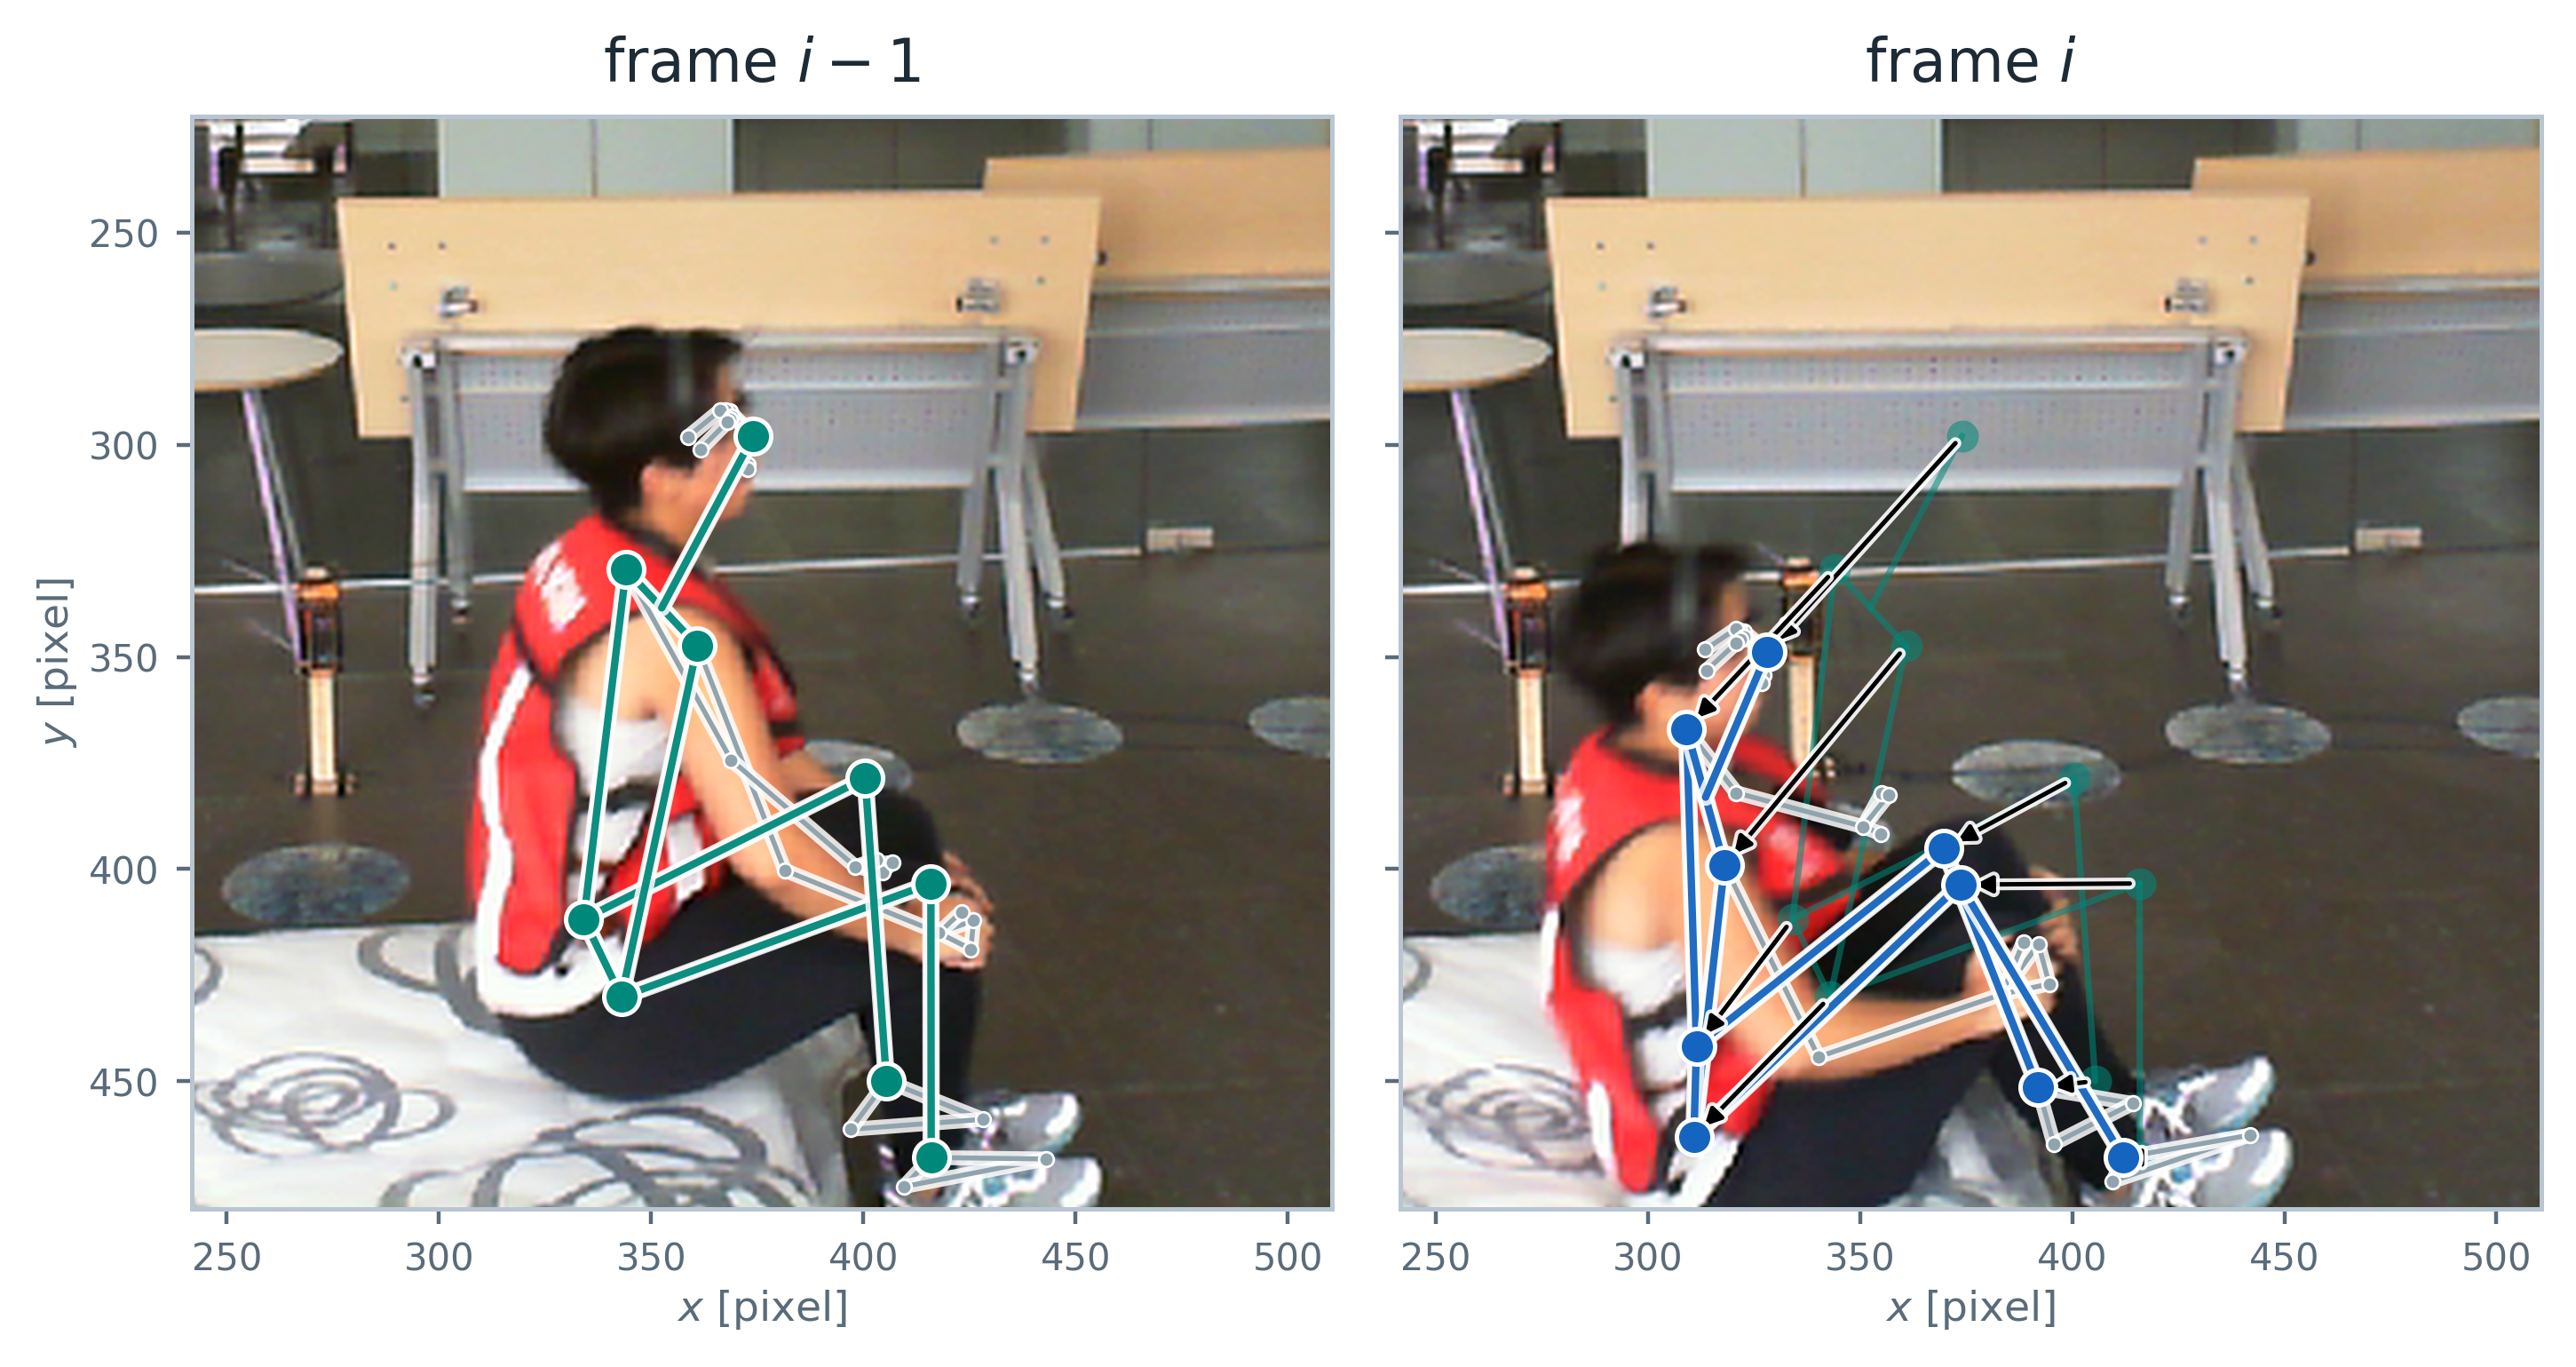
\includegraphics[width=\linewidth]{figure/fig_tracciatore_en.png}
    \caption{Two consecutive frames of a fall (\texttt{sub09\_act05\_trial01}, camera 1, frames 28 and 29). On the left the pose at frame $i-1$; on the right the pose at frame $i$, with the previous one superimposed in transparency}
\label{fig:tracciatore}
\end{figure}

This continuity must, however, be broken when a recording ends. Denoting by $r$ a recording, no previous pose belonging to video $r-1$ must be available at the beginning of the sequence. Using the same notation as Equation~\ref{eq:pose_tracking}, this condition can be expressed as
\begin{equation}
\mathbf{x}^{0,(r)} = \varnothing
\qquad \text{for every } r ,
\label{eq:azzeramento}
\end{equation}

where $\mathbf{x}^{0,(r)}$ denotes the absence of a previous pose at the beginning of recording $r$. Every recording thus starts from an empty state, which is obtained by creating a new estimator at the beginning of each one and closing it at the end. The temporal state is in this way maintained between frames that genuinely belong to the same sequence.
Creating the estimator introduces a few tenths of a second of initialisation, while closing it frees the resources used and prevents the TensorFlow Lite instances from accumulating while the whole archive is processed.

During offline extraction all frames are processed in order, and the program waits for the pose estimation and the computation of the features to be completed before moving on to the next frame.
On the edge device, by contrast, frames arrive continuously from the camera, and the time required for pose estimation determines how many of them can actually be processed.
The processing chain therefore remains the same, but the time constraint changes. This difference is analysed in Chapter~\ref{cap:edge}.

\subsection{Absence of the pose and instability of the coordinates}
\label{sec:posa-mancante}

The landmarks returned by the estimator are not exact measurements of the position of the body, but estimates derived from the image. Their quality can therefore be affected by various factors, such as occlusions, viewpoint or the configuration assumed by the person. Three events may occur:
\begin{enumerate}
    \item the landmark is estimated, but the estimator considers it poorly visible;
    \item the estimator fails to reconstruct a valid pose;
    \item the pose is found, but the coordinates oscillate slightly from one frame to the next.
\end{enumerate}

As regards the first case, MediaPipe returns for each landmark a \emph{visibility} value, associated with the probability that the point is visible in the image \cite{BL}. This value is not used directly in the pipeline: when the pose is available, the geometric engine uses the coordinates of the points needed to build the features.

Visibility was nonetheless analysed over 26.548 frames with a valid pose. Nose, shoulders and hips show median values above $0{,}98$. The situation differs for some points of the limbs: the median visibility of the elbows, for instance, drops from $0{,}81$ to $0{,}52$ when the person is on the ground. The difference is even more marked in lateral recordings: the knee and the ankle on the side further from the camera show values below $0{,}5$ in more than half of the frames, whereas on the side facing the camera they remain around $0{,}9$.

Using visibility as the sole criterion for accepting or rejecting the entire pose did not produce a useful selection. With a threshold of $0{,}5$, all the frames analysed continue to be considered valid, because the main points of the trunk retain very high values. A use of visibility at the level of the individual landmark was not explored in this work. The effect of perturbations applied to the different points is, however, taken up again in Section~\ref{sec:occlusioni}.

The second case concerns the complete absence of the pose. In $4{,}1\%$ of the frames, that is 4.792 cases out of 116.362, the estimator returns no valid pose; the percentage rises to $19\%$ on the external archive examined later. The pipeline identifies these samples through the variable \texttt{ha\_posa}, which equals 1 when the pose is available and 0 when it is absent. In the latter case the features are set to zero, but that value is not treated as a real measurement. Making this distinction is essential, because zero can have a physical meaning: a trunk angle equal to zero, for example, may correspond to a configuration that was actually observed.

When the pose is lost, the temporal state used by the dynamic features is also reset, so as to avoid computing a derivative that compares a sample preceding the loss of tracking with one acquired after tracking has resumed.
The same criterion was applied when building the windows: a window can be constructed only within a continuous stretch, so as not to create sequences that span intervals in which the movement was not actually observed.

The third problem concerns the stability of the coordinates. Even when the pose is available, the landmarks may vary slightly between consecutive frames. Part of this difference is due to the real movement of the person, and part to the uncertainty of the estimate. This phenomenon, known as \emph{jitter}, affects above all the quantities obtained from temporal differences. To quantify it, the displacement of each landmark between two consecutive frames was measured. The displacement of the centre of the hips was subtracted in order to reduce the effect of the overall translation of the person, and the result was normalised with respect to the length of the trunk.

\begin{figure}[htbp]
\centering
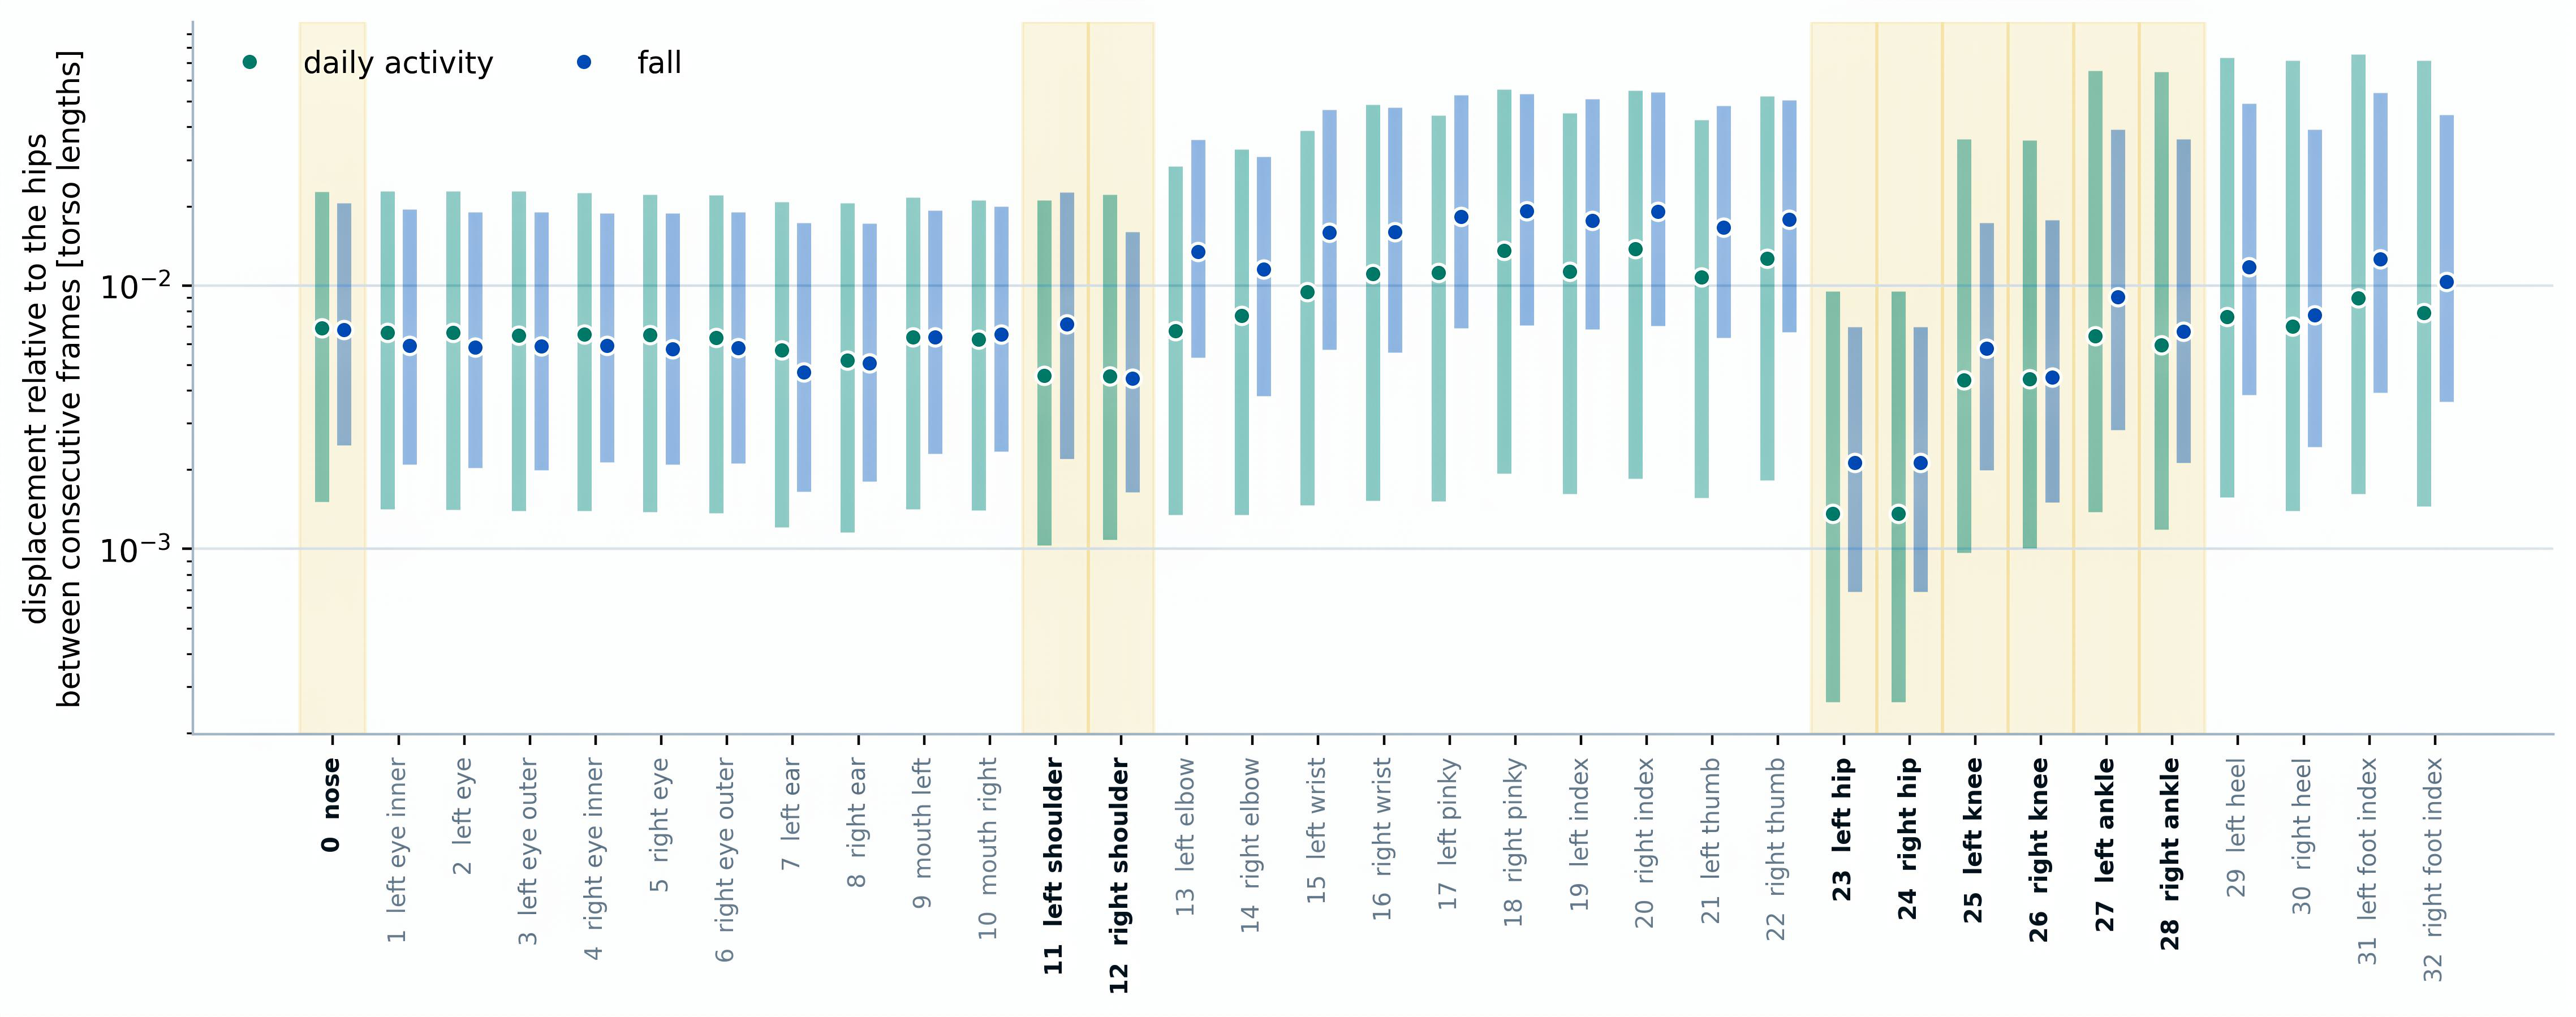
\includegraphics[width=1\textwidth]{figure/fig_spostamento_en.png}
\caption{Displacement of the landmarks between consecutive frames, measured with respect to the centre of the hips and normalised by the length of the trunk.}
\label{fig:spostamento}
\end{figure}

The points of the trunk and of the lower limbs show smaller displacements than the wrists and the fingers. The difference remains visible in the fall recordings as well, where the overall movement increases.
The representations developed rest mainly on the head, the trunk and the lower limbs, and build no features from the landmarks of the hands.

\subsection{Temporal filtering and derivatives}
\label{sec:filtraggio}

One possible remedy for the instability of the landmarks is to apply a temporal filter. During the initial development phase an \emph{Exponential Moving Average} was considered,
\[
\tilde{x}t=
\alpha x_t+
(1-\alpha)\tilde{x}{t-1},
\]

but this option was not subsequently applied to the dataset used in the experiments.
The features are computed directly on the landmarks returned by MediaPipe. In the absence of filtering, the quantities obtained through temporal differences may therefore be more affected by the oscillations. A velocity, for example,
\[
v_i = \frac{x_i-x_{i-1}}{\Delta t_i},
\]
is influenced by the difference between two coordinates, both subject to the uncertainty of the
estimator. Consequently, when the representations were built, only the dynamic quantities considered useful were retained, while the second derivatives present in the earliest versions were removed.

The derivatives retained are computed on the basis of the time that actually elapsed between two consecutive frames. Denoting by $t_i$ the time of the current frame,
\[
\Delta t_i = t_i-t_{i-1}.
\]

In the earliest versions of the pipeline the interval was instead derived from the nominal acquisition frequency. Since, as shown in Section~\ref{sec:cadenza}, the actual cadence is constant neither between recordings nor within a single recording, the final configuration uses the timestamps of the frames directly. In order to describe the movement over a wider time interval as well, some integral quantities were moreover introduced, defined in Section~\ref{sec:integrali}.

\section{Geometric representations of movement}
\label{sec:rappresentazioni}

Once the pose has been estimated, the coordinates of the landmarks must be turned into quantities that describe the configuration and the movement of the person. Three representations of the same movement were built. They do not correspond to different classifiers, but to three different ways of turning the pose into numerical features:
\begin{itemize}
    \item \textbf{A1} works in the image plane and describes mainly the shape and the orientation of the distribution of the landmarks.
    \item \textbf{A2} uses the \emph{world landmarks} supplied by MediaPipe and builds a three-dimensional representation.
    \item \textbf{A3} uses two-dimensional coordinates referred to the geometry of the body, taking the hips as the origin and the length of the trunk as the normalisation factor.
\end{itemize}

The three representations are built before feature selection. The quantities obtained therefore converge into the same set of candidates, and the procedure described in Section~\ref{sec:dtw} establishes which of them to keep in the final representation.
Table~\ref{tab:landmark_rappresentazioni} reports the sets of points needed to build the quantities of the three representations, while Figure \ref{fig:rappresentazioni} shows those sets on a real pose from the dataset, with the index of each point beside the point itself.

\begin{table}[ht]
\centering
\caption{Landmarks used in the three geometric representations.}
\label{tab:landmark_rappresentazioni}
\resizebox{\textwidth}{!}{
\begin{tabular}{llcl}
\toprule
\textbf{Representation} &
\textbf{MediaPipe indices} &
\textbf{No.} &
\textbf{Landmarks used} \\
\midrule
A1 & 0, 11, 12, 23, 24, 27, 28
   & 7 & nose, shoulders, hips, ankles \\
A2 & 0, 11, 12, 23, 24
   & 5 & nose, shoulders, hips \\
A3 & 0, 11, 12, 23--28
   & 9 & nose, shoulders, hips, knees, ankles \\
\bottomrule
\end{tabular}
}
\end{table}

\begin{figure}[htbp]
    \centering
    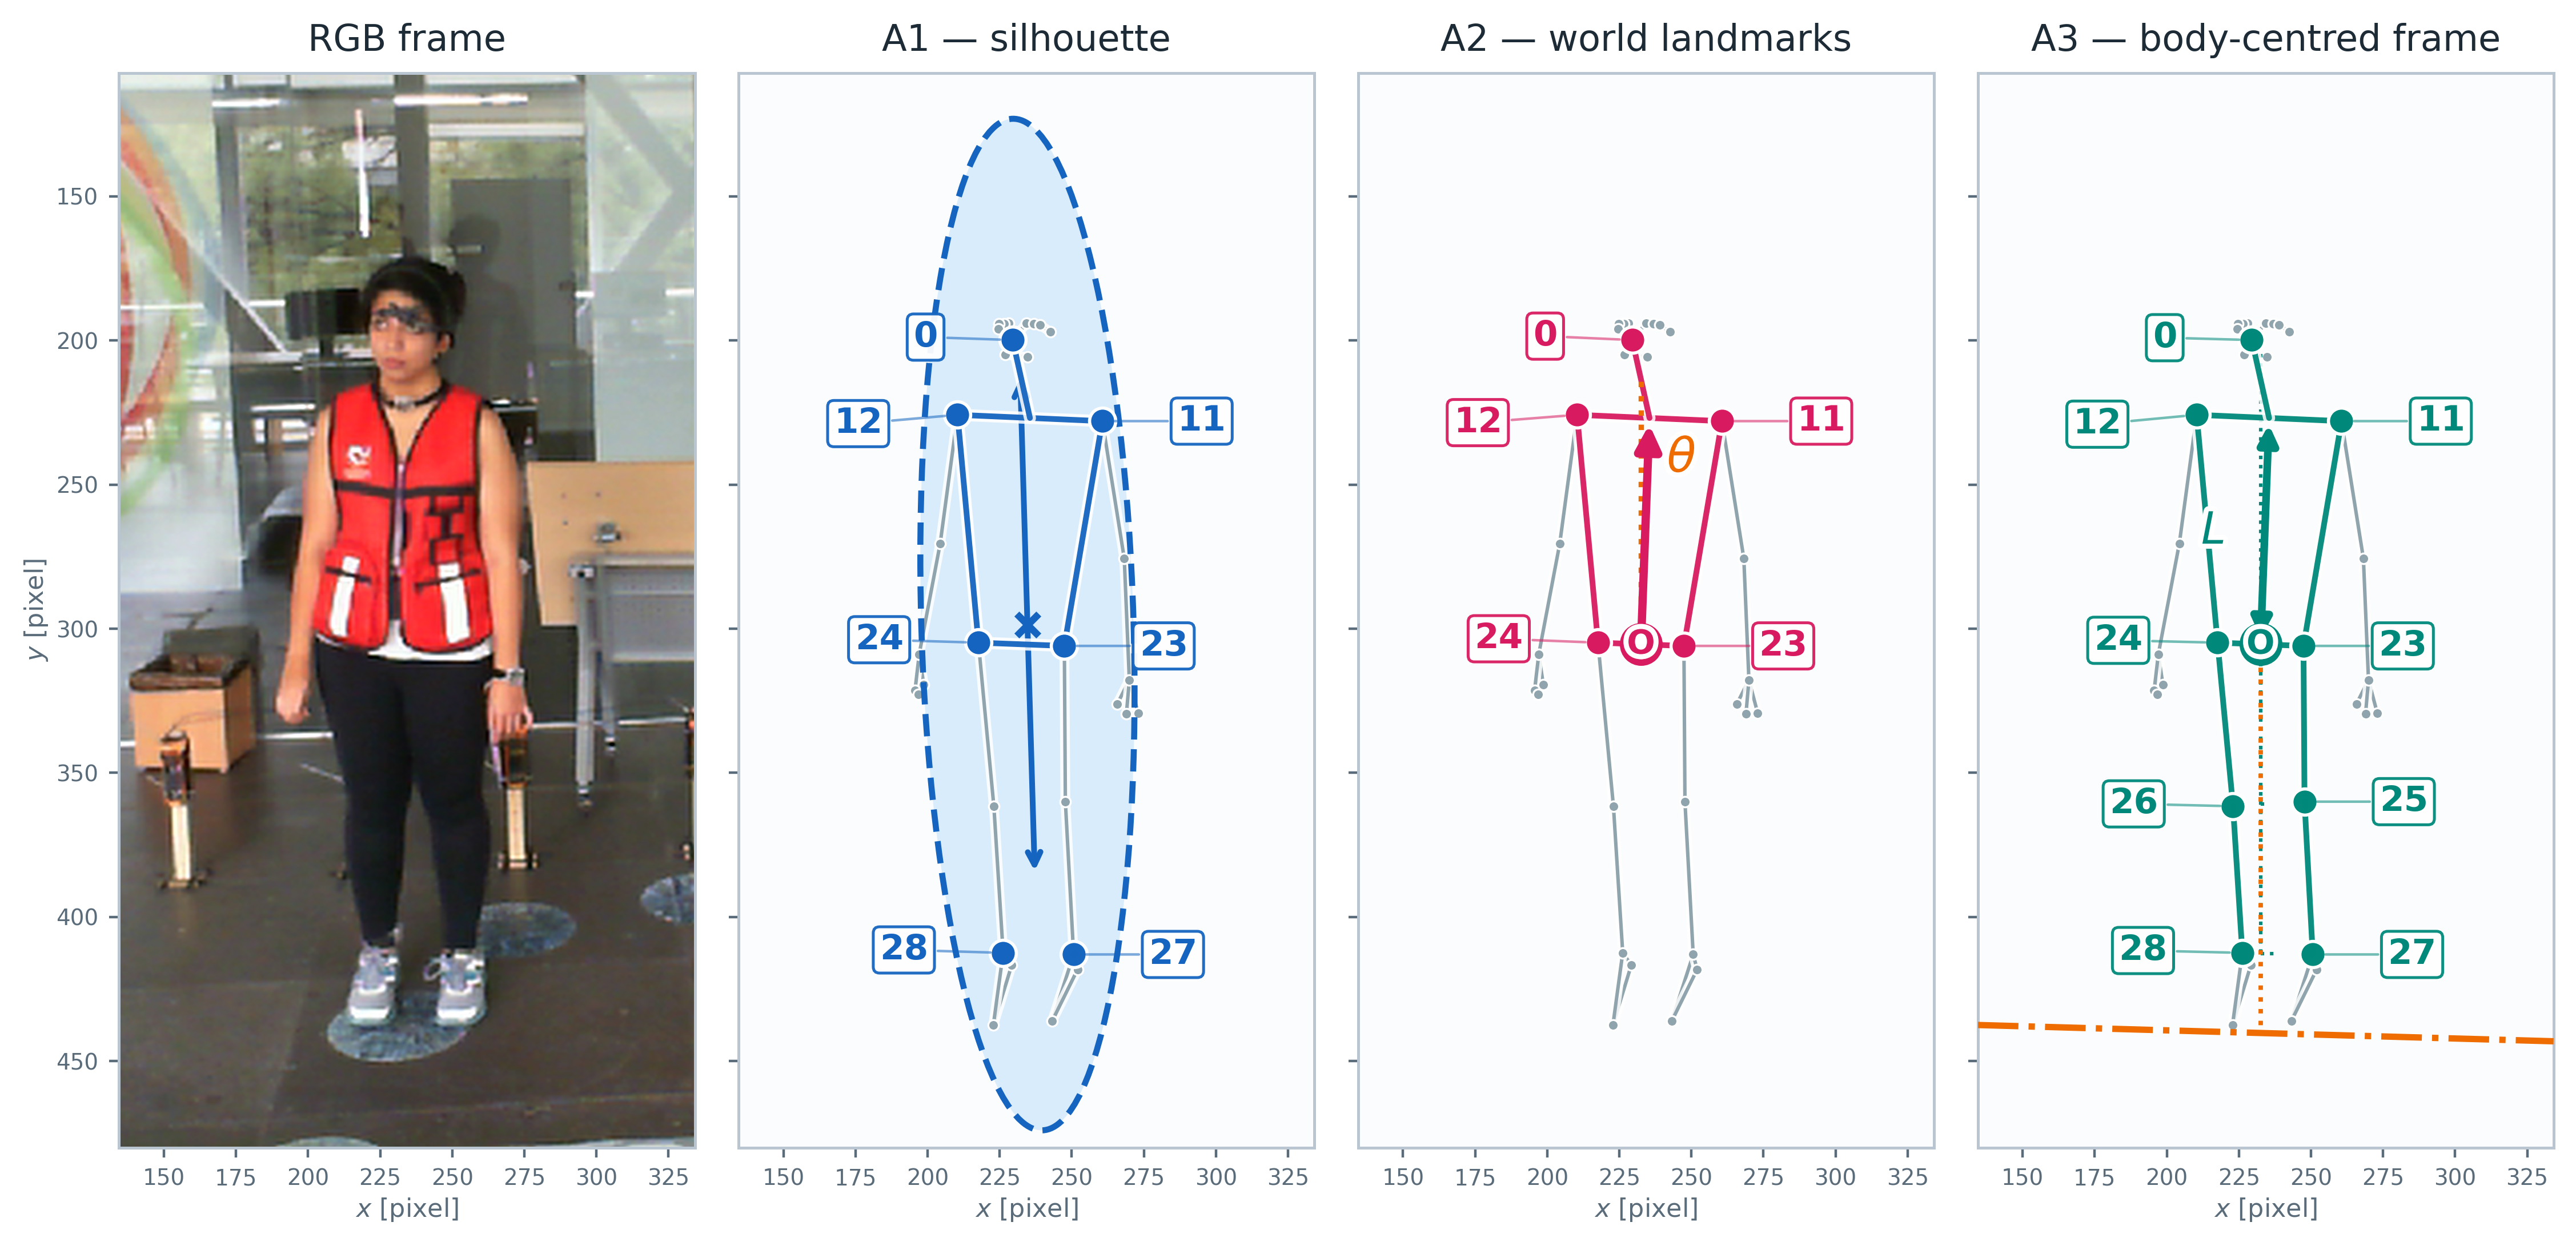
\includegraphics[width=1\linewidth]{figure/fig_landmark_en.png}
    \caption{The set of landmarks of the three representations}
    \label{fig:rappresentazioni}
\end{figure}

\subsection{A1: description of the silhouette in the image plane}

Representation A1 uses the landmarks listed in Table \ref{tab:landmark_rappresentazioni} as a distribution of points in the image plane. The anatomical connections are not used directly, because what matters is the overall shape assumed by the body. From a geometric point of view, this cloud can be described by an ellipse, where the major axis represents the dominant orientation of the body, the minor axis the dispersion in the orthogonal direction, and the ratio between them describes its elongation.

The ellipse is derived from the covariance matrix of the landmarks. Denoting by $J$ the set of points used and by $p_j\in\mathbb{R}^2$ the position in pixels of point $j$, the centre of the distribution is computed:
\begin{equation}
\bar{p} =
\frac{1}{|J|}
\sum_{j\in J} p_j .
\label{eq:centroide_a1}
\end{equation}

The covariance matrix is
\begin{equation}
S =
\frac{1}{|J|-1}
\sum_{j\in J}
\left(p_j-\bar{p}\right)
\left(p_j-\bar{p}\right)^{\top}.
\label{eq:covarianza}
\end{equation}

which makes it possible to identify the two principal directions of the point cloud through its eigenvalues and eigenvectors:
\begin{equation}
S\,v_k = \lambda_k v_k,
\qquad
\lambda_1 \geq \lambda_2 \geq 0,
\qquad
v_1 \perp v_2 .
\label{eq:autovalori}
\end{equation}

The eigenvector $v_1$ describes the direction along which the body is most widely distributed, while the eigenvector $v_2$ identifies the orthogonal direction. The dimensions along the two axes are
\begin{equation}
a = \sqrt{\lambda_1},
\qquad
b = \sqrt{\lambda_2},
\label{eq:assi_a1}
\end{equation}

The ratio
\begin{equation}
\rho = \frac{a}{b}
\label{eq:allungamento_a1}
\end{equation}
measures how elongated or compressed the configuration appears, while the inclination of the principal axis is obtained from
\begin{equation}
\theta =
\operatorname{atan2}\left(v_{1y},v_{1x}\right).
\label{eq:angolo_a1}
\end{equation}

Nine quantities are extracted from A1: \textbf{the two semi-axes $a$ and $b$; the ratio $\rho=a/b$; the inclination $\theta$ of the principal axis, expressed in degrees; the temporal variations of $a$, of $\rho$ and of $\theta$; the horizontal and vertical components of the velocity of the centre $\bar{p}$, normalised with respect to the dimensions of the image.}

The example reported in Figure~\ref{fig:momenti_a1} shows the geometric meaning of the representation at two moments of the same fall. In an upright position the ellipse is oriented mainly vertically; when the person is on the ground, the principal axis instead takes on an almost horizontal direction.
\begin{figure}[htbp]
\centering
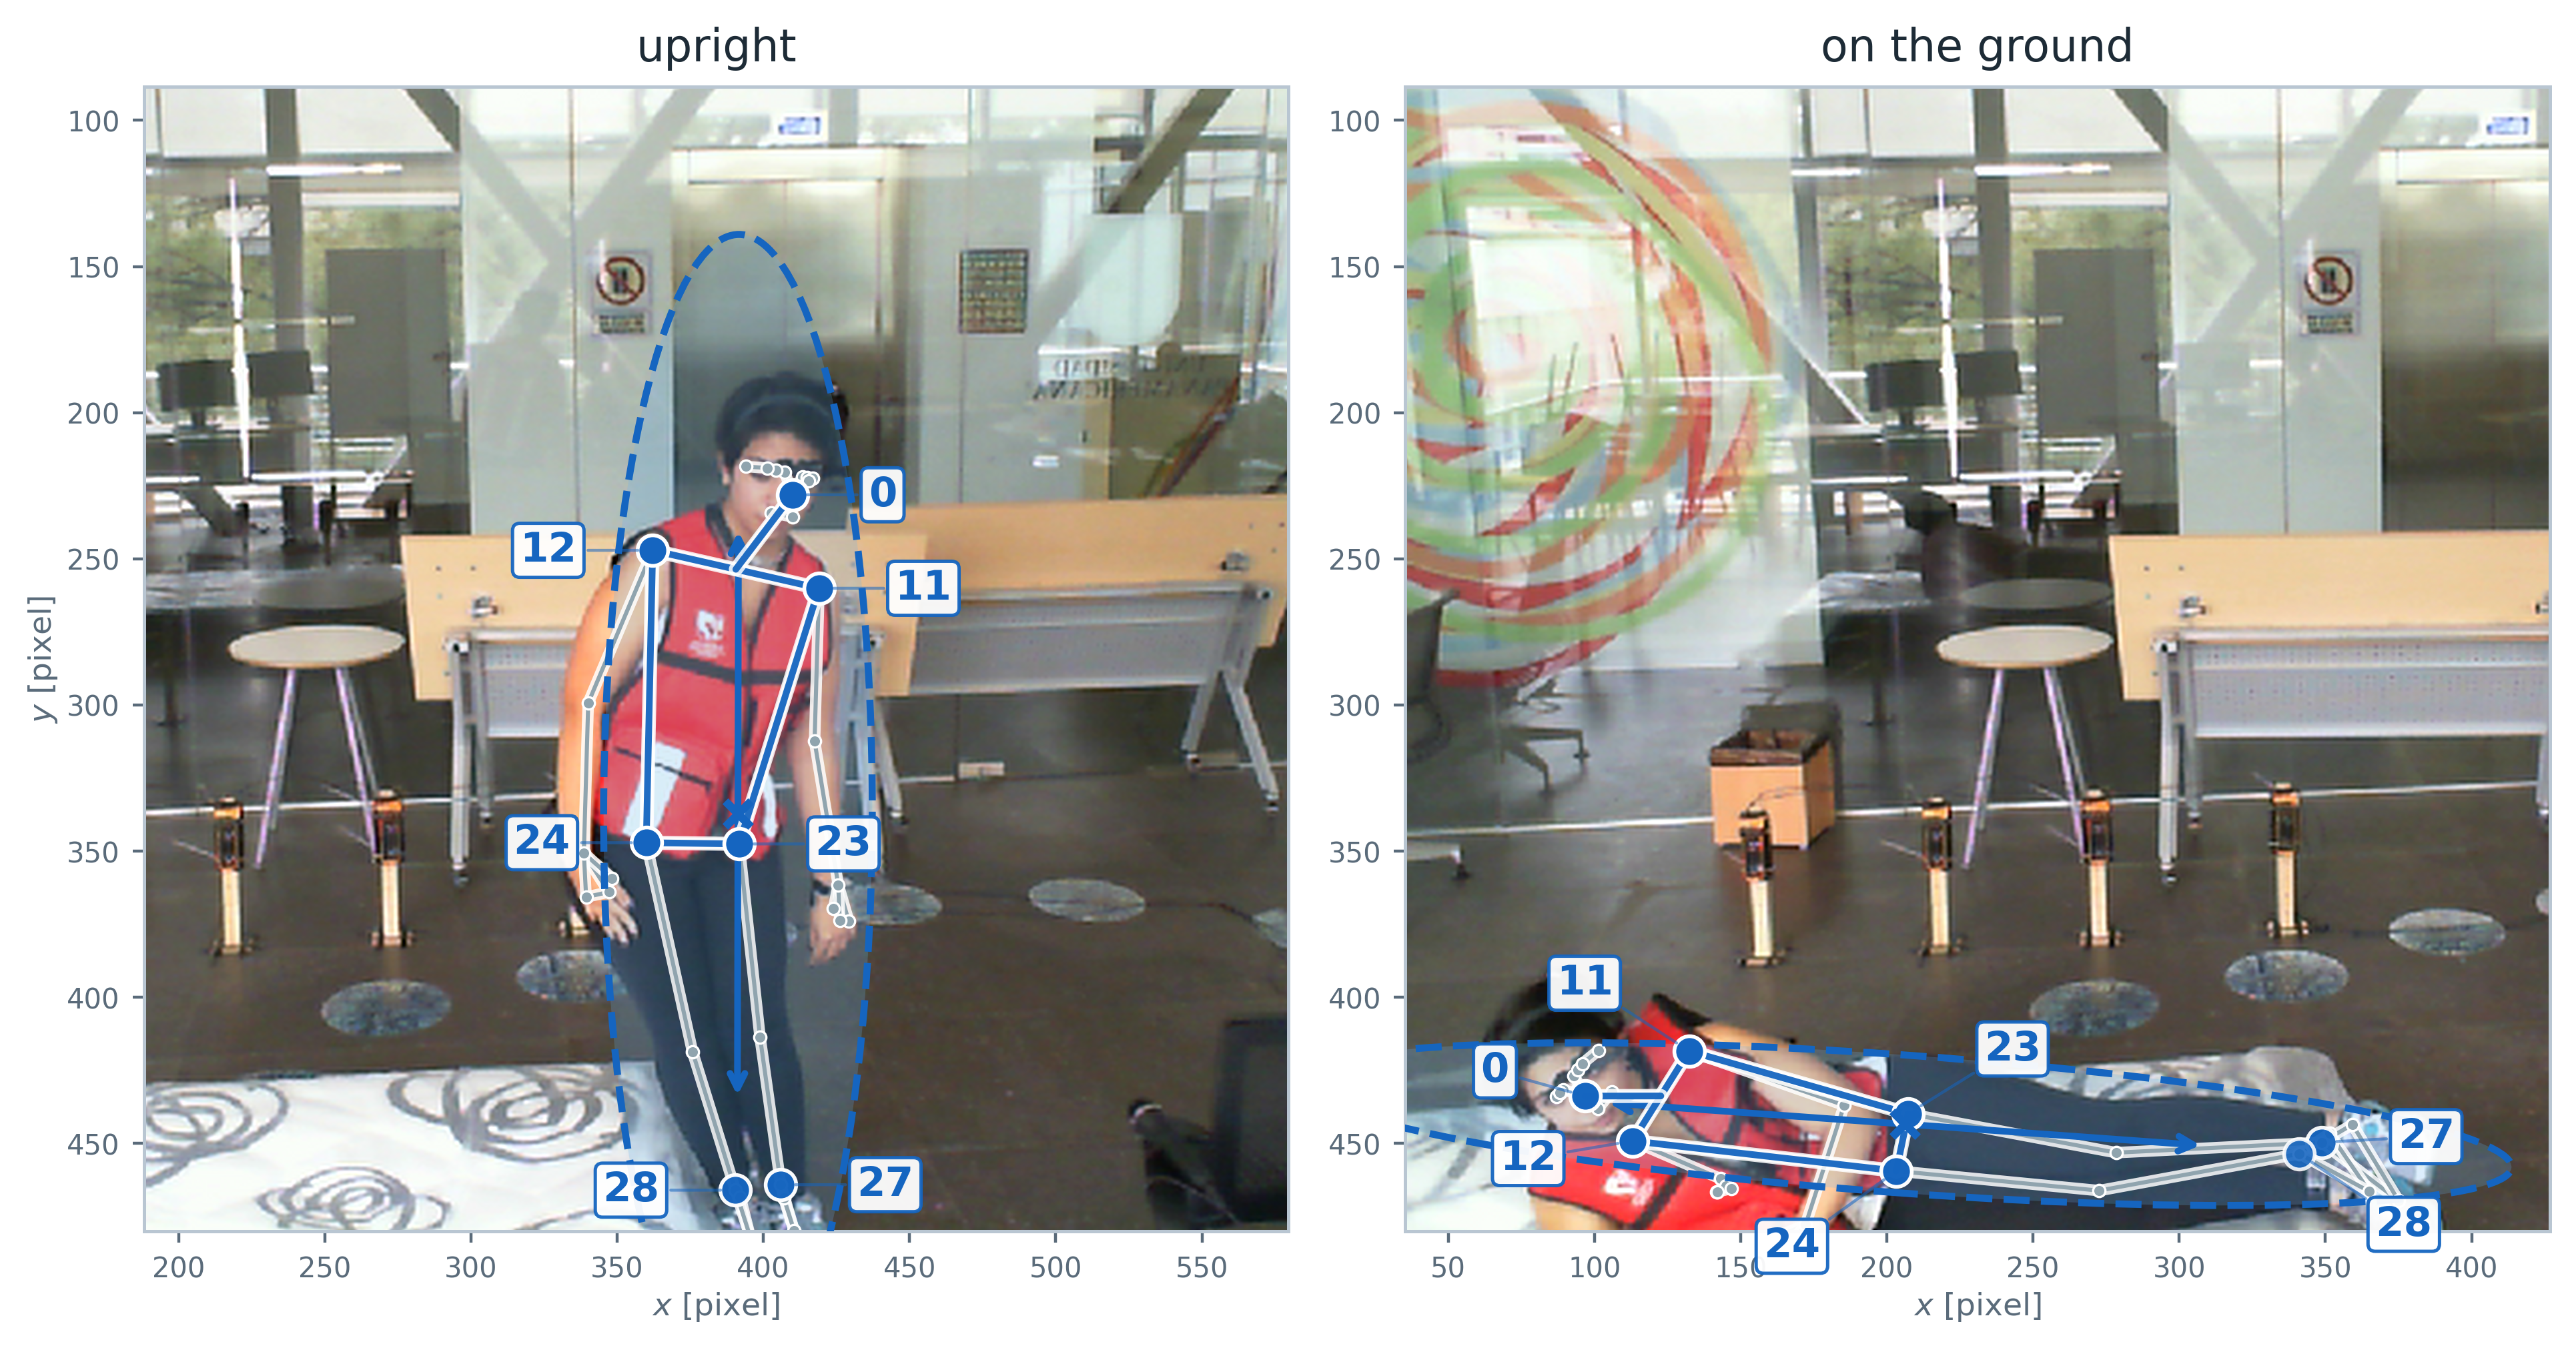
\includegraphics[width=\textwidth]{figure/fig_momenti_a1_en.png}
\caption{Representation A1 at two instants of the same fall
(\texttt{sub09\_act04\_trial01}, camera 1).}
\label{fig:momenti_a1}
\end{figure}

The main limitations of A1 stem from the fact that all the quantities are computed in the plane of the image. The same posture may therefore look different when the viewpoint of the camera changes; and because the principal axis of the ellipse has no direction, an axis oriented at $30^\circ$ is equivalent to the same axis represented at $210^\circ$. The orientation therefore has a periodicity of $180^\circ$. Before its temporal variations are computed, the angle is therefore unwrapped so as to account for that periodicity, avoiding numerical jumps in depth.

\subsection{A2: three-dimensional description}

Representation A2 uses the \emph{world landmarks}, again those listed in Table \ref{tab:landmark_rappresentazioni}. Unlike the coordinates in the image plane, every point is described by three coordinates and therefore also retains information about depth.
The main quantities are built starting from the trunk vector. Denoting by
$p_{s_L}$ and $p_{s_R}$ the two shoulders and by $p_{h_L}$ and $p_{h_R}$ the two hips, the respective midpoints are computed

\begin{equation}
p_s = \frac{p_{s_L}+p_{s_R}}{2},
\qquad
p_h = \frac{p_{h_L}+p_{h_R}}{2}.
\end{equation}

The vector $t = p_s-p_h $ describes the direction of the trunk in three-dimensional space.
The five quantities derived from this representation are:\textbf{trunk angle, variation of the trunk angle, magnitude of the angular velocity of the trunk, velocity of the head and vertical position of the head with respect to the hips.} Figure~\ref{fig:momenti_a2} shows the trunk vector at the same two instants used for A1.

\begin{figure}[htbp]
\centering
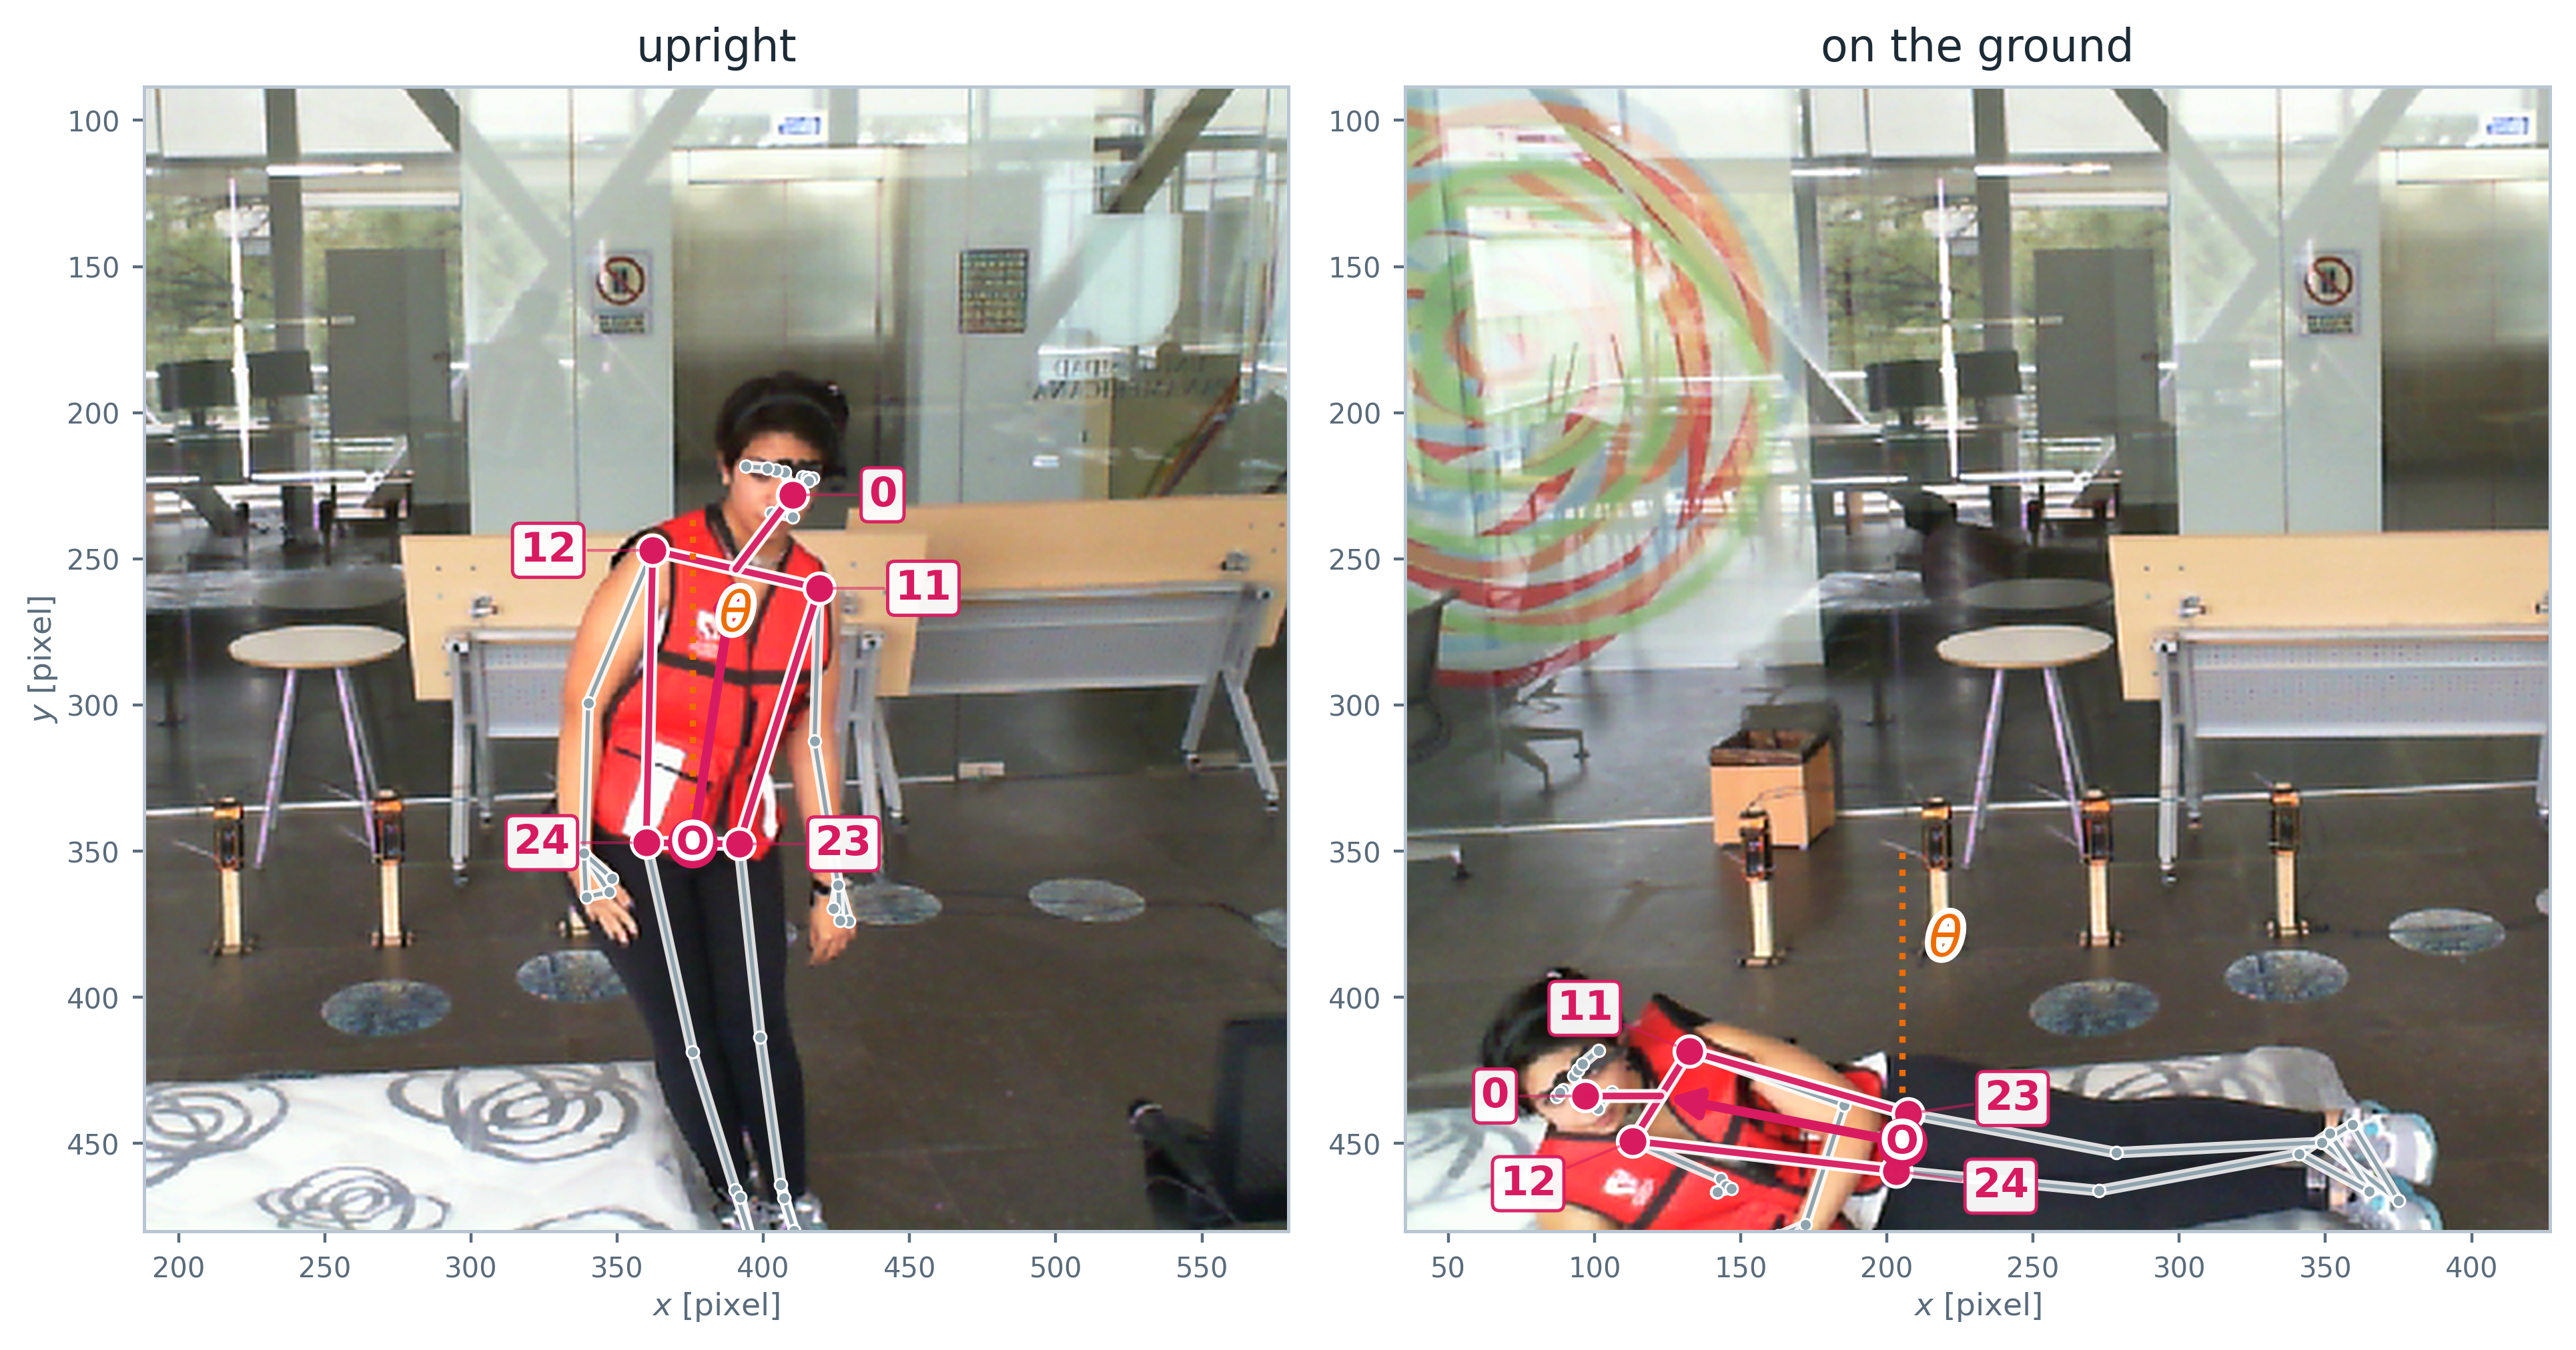
\includegraphics[width=\textwidth]{figure/fig_momenti_a2_en.png}
\caption{Representation A2. The angle goes from $8{,}96^\circ$ in an upright position to $-79{,}13^\circ$ on the ground. The point O marks the centre of the hips, the origin of the reference system of the \emph{world landmarks}.}
\label{fig:momenti_a2}
\end{figure}

The \emph{world landmarks} must, however, be interpreted with respect to their own reference system, which is centred on the hips and does not coincide with an absolute coordinate system of the room. Consequently, the trunk angle does not represent an absolute inclination with respect to the floor or to the direction of gravity. This characteristic is most apparent in the position of the hips which, being the origin of the reference system, remains practically constant by construction. Over forty consecutive frames the standard deviation of its position is $3\cdot10^{-5}$ metres for the hips, against about $1{,}75\cdot10^{-2}$ metres for the nose.

The quantities relating to the translation of the hips, present in the initial formulation, were therefore measuring mainly numerical variations and were removed. For the same reason, in the integral quantities of A2 the nose is followed rather than the centre of the hips.

\subsection{A3: description referred to the geometry of the body}

Representation A3 again uses two-dimensional landmarks, but expresses them with respect to the geometry of the person. The centre of the hips is taken as the origin of the reference frame, while the distance between the centre of the hips and the centre of the shoulders defines the length of the trunk. Denoting by $p_j(i)$ the position of landmark $j$ in frame $i$, by $p_{\text{bacino}}(i)$ the centre of the hips and by
$L_{\text{tronco}}(i)$ the length of the trunk, the normalised position is

\begin{equation}
P_j(i) =
\frac{p_j(i)-p_{\text{bacino}}(i)}
{L_{\text{tronco}}(i)} .
\label{eq:normalizzazione}
\end{equation}

The position of the points with respect to the body is described by subtracting the centre of the hips, while the division by the length of the trunk reduces the effect of the apparent scale. Consequently the distances obtained are no longer in pixels, but in trunk lengths. If a person moves closer to the camera, for example, both the distances between the landmarks and the apparent length of the trunk increase. Their ratio varies far less, and so describes the relative configuration of the various parts of the body.

Starting from the landmarks listed in Table~\ref{tab:landmark_rappresentazioni}, the nine quantities of A3 are: \textbf{length of the trunk, trunk angle and its temporal variation, relative height of the head, relative height of the knees, relative height of the ankles, normalised width of the body, velocity of the hips and velocity of the head with respect to the hips.}

A3 therefore introduces detail about the arrangement of the different parts of the body. In particular, the use of knees and ankles can help to distinguish body configurations that have a similar trunk orientation. Figure~\ref{fig:momenti_a3} shows the reference frame used at the two instants already considered for A1 and A2.

\begin{figure}[htbp]
\centering
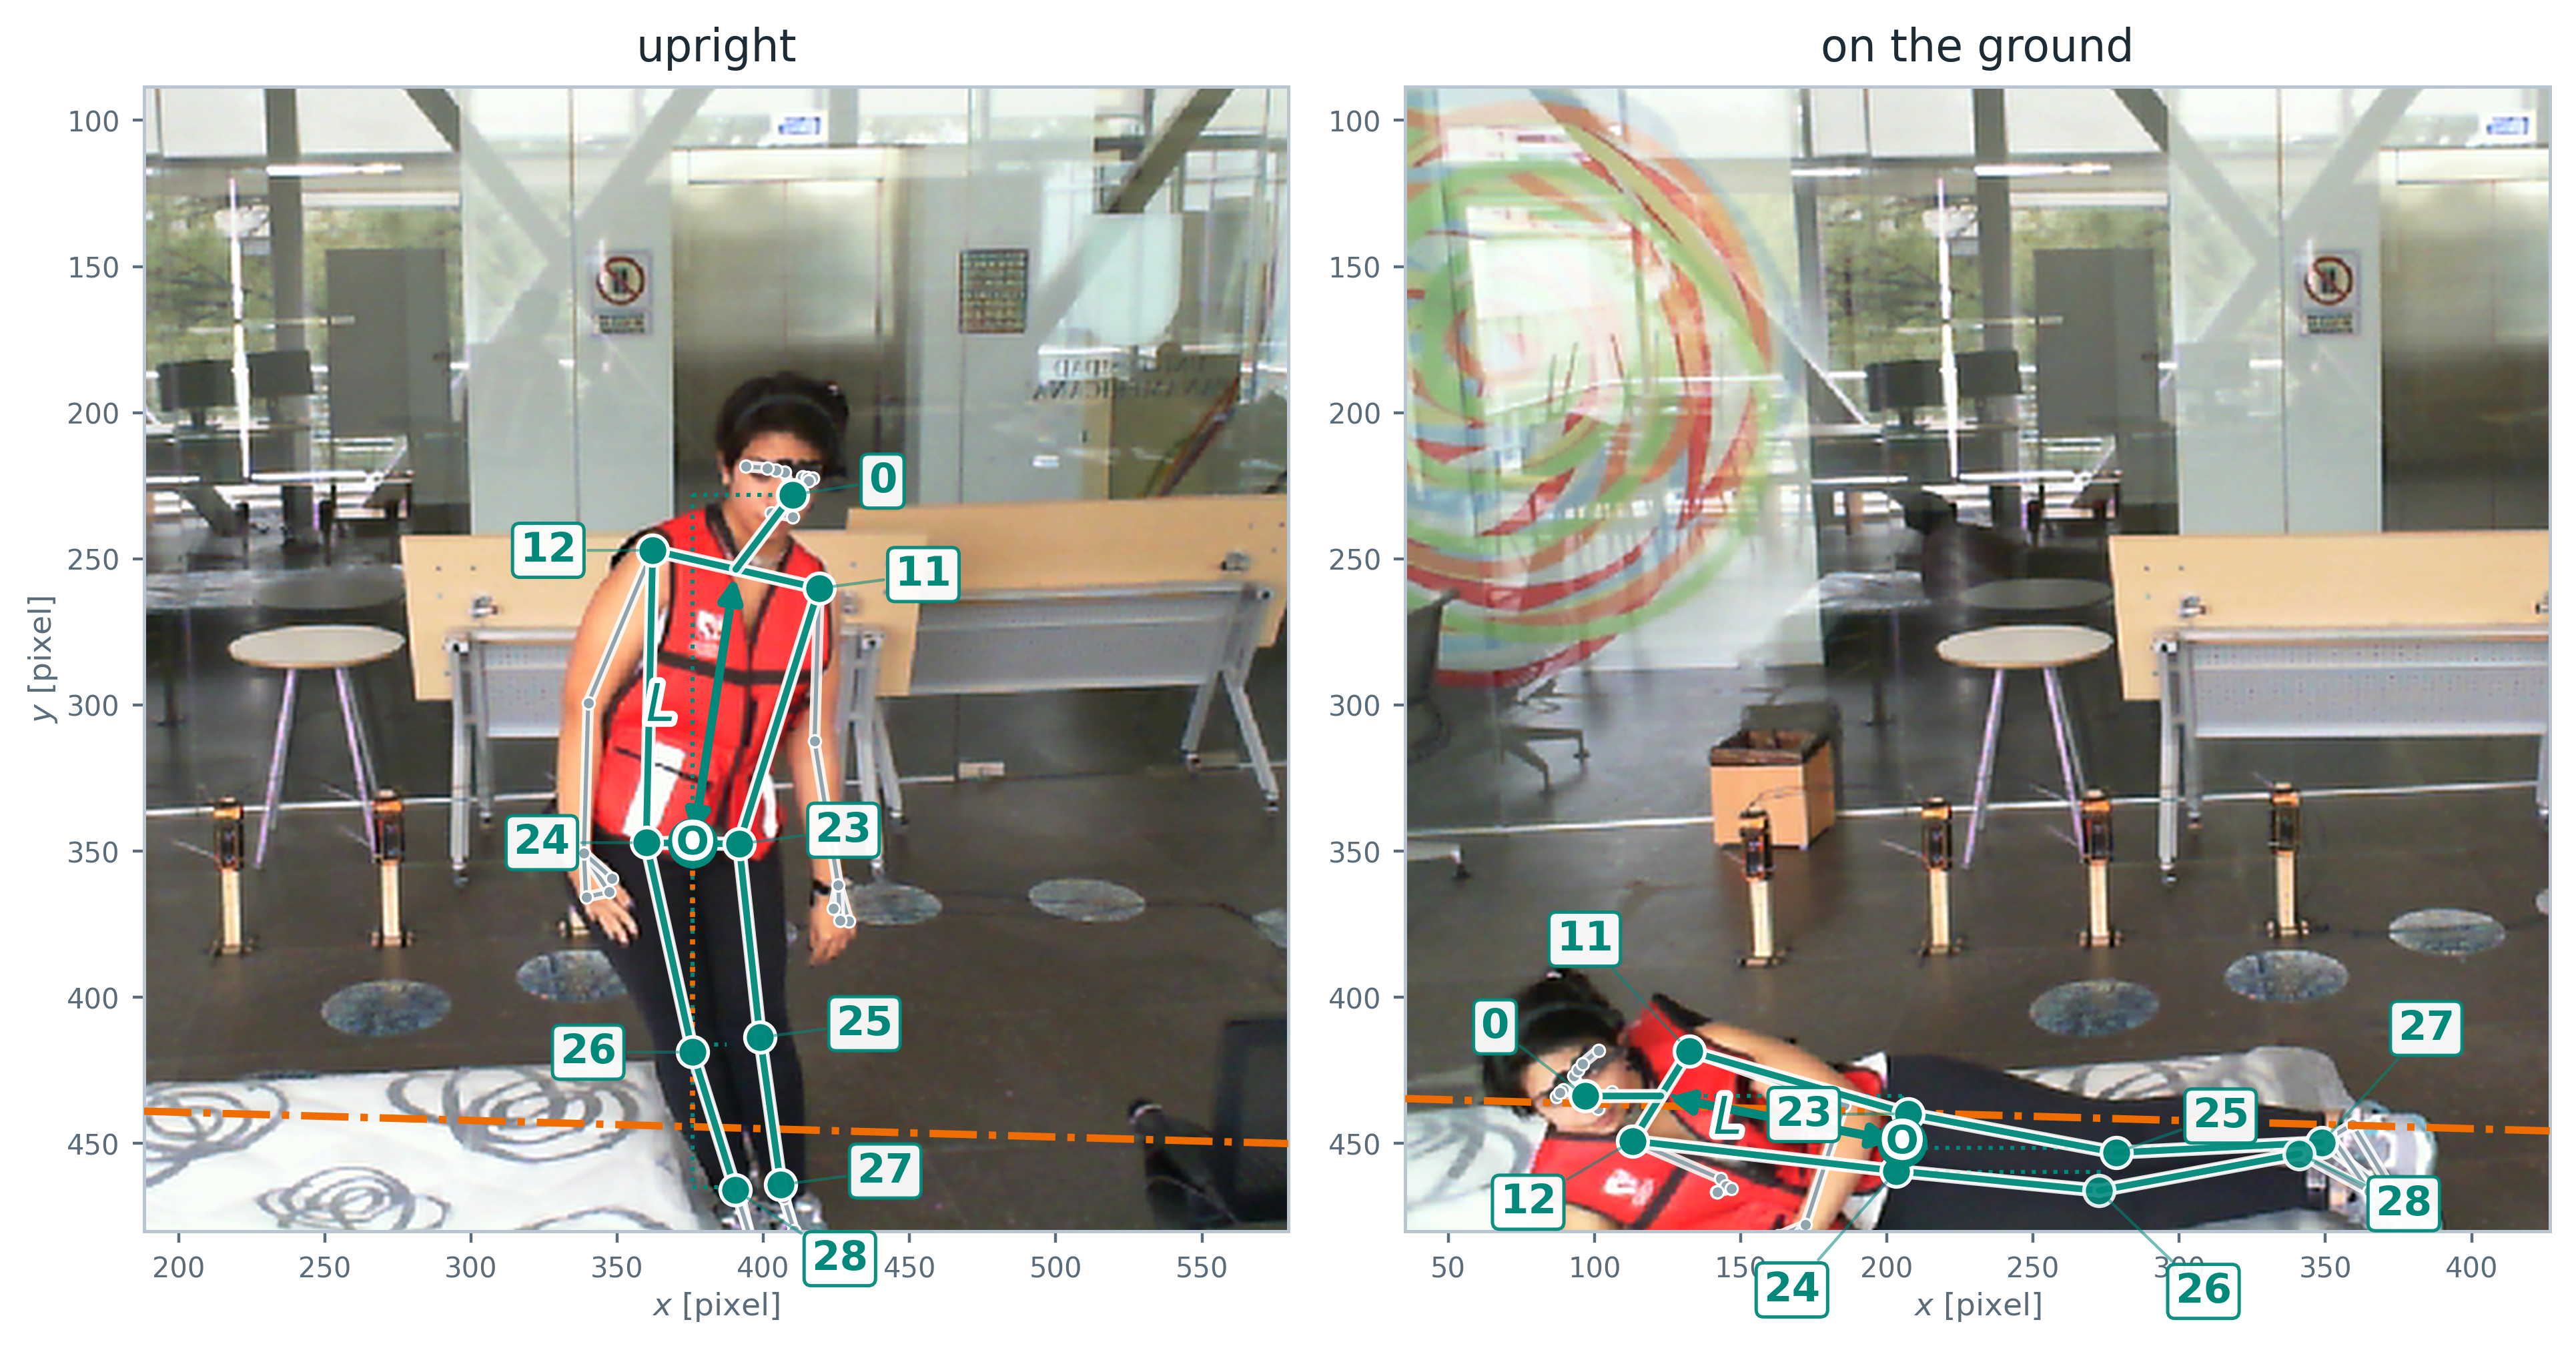
\includegraphics[width=\textwidth]{figure/fig_momenti_a3_en.png}
\caption{Representation A3 at the same two instants as
Figures~\ref{fig:momenti_a1} and~\ref{fig:momenti_a2}. The point O marks the
centre of the hips, used as the origin of the reference frame, while $L$
represents the length of the trunk used to normalise the distances.}
\label{fig:momenti_a3}
\end{figure}

The normalisation reduces the dependence on translation and scale, but does not eliminate the one due to perspective. Moreover, by referring the landmarks to the hips, the information about the absolute position of the person in the environment is lost. A person lying on the floor and one lying on a bed can generate very similar body-centric configurations. In order to recover this information, Section~\ref{sec:pavimento} will introduce the position of the hips with respect to the floor, estimated from the scene. Taken together, the three representations described provide 23 basic geometric and kinematic quantities: nine belonging to A1, five to A2 and nine to A3.

\section{Integral quantities for the description of movement}
\label{sec:integrali}

The representations described in the previous section comprise both static quantities and dynamic quantities obtained through differences between consecutive frames. As discussed in Section~\ref{sec:filtraggio}, the coordinates are estimates and show small oscillations even when the real position of the body varies little. In order to provide a description of the movement over a wider time interval, three integral quantities were introduced.

\subsection{Definition of the integral quantities}

The quantities are computed over a sliding window containing the last \(K\) frames. Denoting by
\[
W_t=\{t-K+1,\ldots,t\}
\]
the window considered, by \(\theta_t\) the orientation of the trunk and by \((x_t,y_t)\) the position of the point being followed, the following are defined:

\begin{align}
\text{escursione}_t &= \max_{\tau \in W} \theta_\tau
                     - \min_{\tau \in W} \theta_\tau
                     \label{eq:escursione}\\[4pt]
\text{percorso}_t   &= \frac{1}{s}\sum_{\tau \in W}
                       \sqrt{(x_\tau - x_{\tau-1})^2 + (y_\tau - y_{\tau-1})^2}
                     \label{eq:percorso}\\[4pt]
\text{discesa}_t    &= \frac{1}{s}\Big( y_t - \min_{\tau \in W} y_\tau \Big)
                     \label{eq:discesa}
\end{align}

The three features describe different aspects of the movement. The \emph{excursion} measures how much the orientation of the trunk varies within the window, the \emph{path} the distance covered overall by the point being followed, and the \emph{descent} how far below the highest recently observed position the current point lies.

The factor \(s\) is used to normalise the distances. For A1 it is derived from the size of the silhouette, while for A2 and A3 the length of the trunk is used. In this way the quantities depend less on the apparent size of the person in the image.

The point being followed also changes according to the representation:
\begin{itemize}
    \item A1: centroid of the set of landmarks,
    \item A2: nose in the \emph{world landmarks}.
    \item A3: centre of the hips in the image plane,
\end{itemize}

Accumulating over several samples does not eliminate the noise of the landmarks. In the path, for instance, distances that are always positive are summed, and so any oscillations may increase the distance covered rather than cancelling out. Excursion and descent can likewise be affected by outliers, since they depend on the maximum, the minimum, or both. The advantage is that they describe the movement on a wider time scale instead of depending solely on the variation between two consecutive frames. The resulting signal is therefore more regular, while remaining sensitive to the errors introduced by pose estimation.

\begin{figure}[ht]
\centering
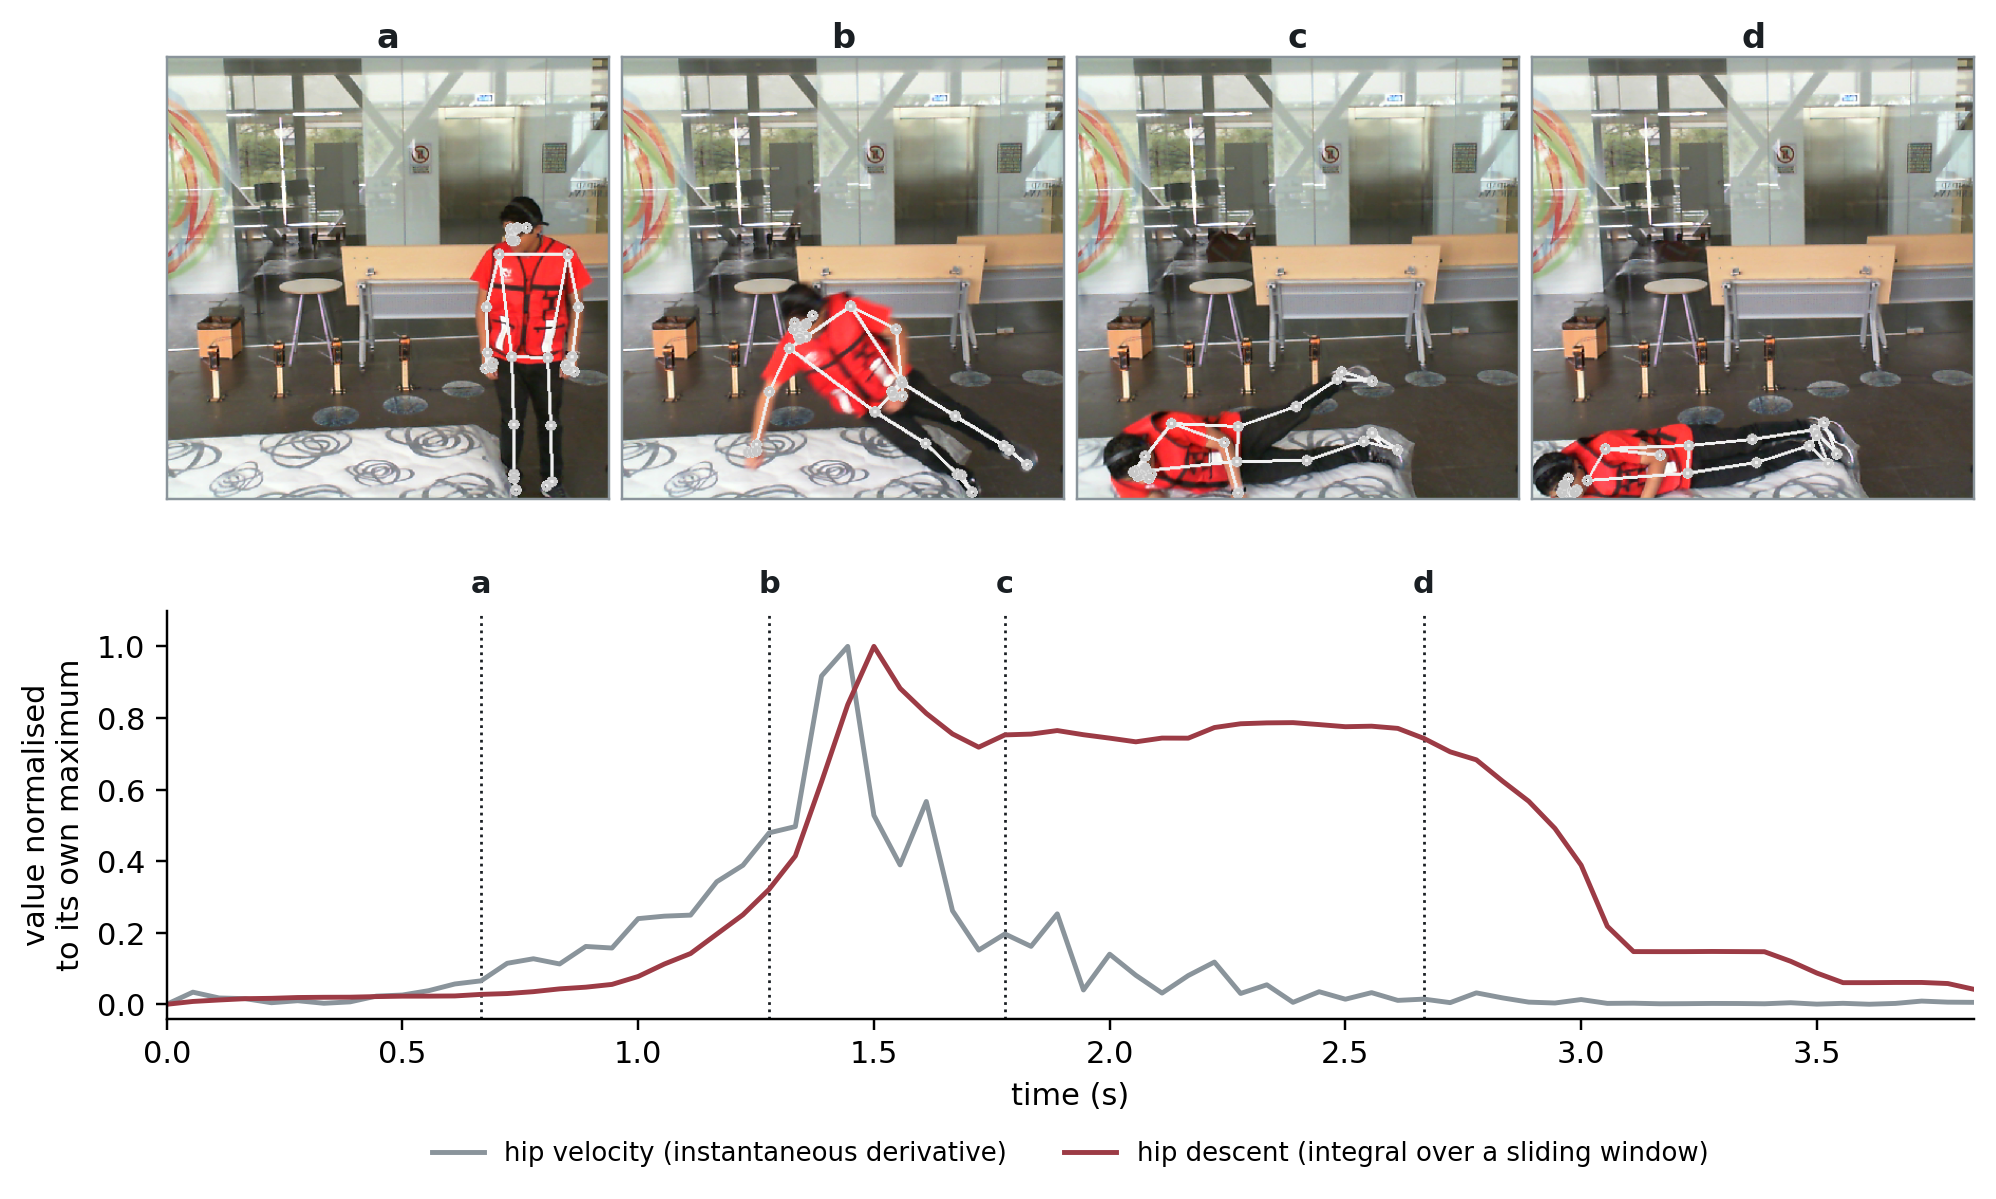
\includegraphics[width=\textwidth]{figure/fig_striscia_en.png}
\caption{Comparison between an instantaneous quantity and an integral quantity during a fall.} \label{fig:striscia}
\end{figure}

Figure~\ref{fig:striscia} shows the contrast on a single fall. The two quantities rise together and reach their maximum during the transition: the derivative is no less sensitive to the event. As soon as the body comes to rest, the velocity of the hips collapses, going from $3{,}76$ at instant (b) to $0{,}11$ at instant (d), while the accumulated descent rises to $1{,}40$ and stays there, decaying only when the accumulation window leaves the event.

\subsection{Causal computation and choice of the length $K$}

The quantities defined in Equations~\eqref{eq:escursione}--\eqref{eq:discesa} can be computed in two ways. In offline processing they could be computed by sliding a window over the whole sequence, which is already available. That solution would not, however, be directly usable on the edge device, where the frames arrive one at a time and no information later than the current instant is available.

In order to use the same logic in both conditions, the pipeline keeps a circular buffer containing the last \(K\) samples and, at every new frame, updates the three integral quantities using only the information already observed. The computation is therefore causal and is applied in the same way both during offline extraction and during execution on the device.
If the pose is lost, the buffer is reset. This prevents the accumulation from spanning an interval in which the movement of the person was not monitored. After start-up, or after a loss of the pose, the buffer must therefore fill up again before the whole expected history is available.

The length of the buffer determines how much recent movement enters the computation. With a small value a shorter interval is observed and the representation is more responsive, but little noise is attenuated. Increasing \(K\) means that a longer portion of the sequence is considered, but a brief event may end up spread over a larger number of samples. The value adopted is
\[
K=31.
\]
At the nominal frequency of 18 frames per second, 31 samples correspond to about
\[
\frac{31}{18}\simeq 1{,}72\text{ s}.
\]

\(K\) denotes, however, a number of samples and not a fixed duration. Considering the frequencies actually measured in the dataset, 31 frames cover roughly between 1,58 and 2,15~s. On the edge device, where the processing frequency may be lower, the same number of samples may therefore represent an even longer time interval. This misalignment is analysed in Chapter~\ref{cap:edge}.

The buffer moreover requires an initial warm-up period: in the first \(K\) frames after start-up the quantities do not yet have the whole history required, and the same happens after a loss of the pose, since the buffer is reinitialised. The value \(K=31\) is retained in the configuration used in the experiments. The effect of different values is assessed in the following chapters, together with the consequences for the operation of the system in a real environment.
The three quantities are computed for A1, A2 and A3. Nine are therefore added to the 23 basic geometric and kinematic quantities, bringing the overall number of candidate features to \textbf{32}.

\subsection{Assessment of temporal regularity}
\label{sec:regolarita}

In order to compare the regularity over time of the instantaneous quantities and of the integral ones, the one-step autocorrelation was measured, that is the correlation between the value of a quantity at time \(t\) and its value at the previous sample:
\[
\rho_1 = \frac{\operatorname{Cov}\big(x_t,\,x_{t-1}\big)}
              {\sigma_{x_t}\,\sigma_{x_{t-1}}}.
\]

The computation considers only pairs of consecutive samples belonging to continuous stretches in which the pose is available. If tracking is lost, the samples lying on either side of the interruption are not related to each other.

The autocorrelation describes how far the value of a quantity tends to stay similar between two consecutive samples. A high value of \(\rho_1\) indicates that the quantity tends to change more gradually, while lower values indicate more rapid variations.
This measure was used only to compare the temporal regularity of the signals. It cannot establish whether a feature is more useful for distinguishing a fall from an ordinary daily activity. The values obtained and the comparison between the two families of quantities are reported in Section~\ref{sec:autocorrelazione} of the experimental chapter.

\subsection{Robustness and limitations}
\label{sec:robustezza}

The three integral quantities nonetheless depend on the coordinates produced by the pose estimator. In order to verify how far small variations of the landmarks can affect performance, a test was carried out by adding independent Gaussian noise to the coordinates.

Denoting by \(p\) a coordinate of the landmark, the perturbed value is
\[ \tilde{p}=p+\varepsilon,
\]
with
\[ \varepsilon \sim \mathcal{N} \left(0,\left(\sigma L_{\text{tronco}}\right)^2\right),
\]
where \(L_{\text{tronco}}\) is the length of the trunk and \(\sigma\) denotes the relative intensity of the noise. The standard deviation of the noise is therefore expressed as a fraction of the length of the torso, so that the intensity of the perturbation does not depend on the size of the person in the image.
The test is repeated using
\[
\sigma \in \{0,\;0{,}005,\;0{,}010,\;0{,}020,\;0{,}040\}.
\]
For every level, three sets of features are compared: the representation without the integral quantities, the complete one with the integral quantities, and the subset selected by DTW. The results are reported in Section~\ref{sec:rumore}.

This test describes, however, only small random and independent perturbations of the coordinates. In some domestic recordings a different behaviour was also observed: in the presence of occlusions, or when the person is very close to the camera, the estimator may switch between alternative configurations of the same pose and keep the wrong configuration for several frames.

An error that is coherent over time may be interpreted by the integral quantities as real movement. The behaviour is also analysed on the domestic recordings, comparing the excursion of the trunk computed over the sliding window in sequences where the person remains still on a sofa and in sequences containing a fall. Using a time window therefore reduces the dependence on instantaneous differences, but does not eliminate the dependence on the correctness of the pose. The quantitative verification is discussed together with the noise test in Section~\ref{sec:rumore}.

\section{Estimating the height of the hips above the floor}
\label{sec:pavimento}

Representation A3 normalises every quantity with respect to the centre of the hips and to the length of the trunk. This choice reduces the dependence on the position and on the scale of the person in the image, but loses the information about their absolute position in the scene.
The limitation shows itself when similar postures occur at different heights. A person lying on a bed or on a sofa may have a body configuration very similar to that of a person who has remained on the ground after a fall. Body-centric coordinates alone describe the posture well, but cannot tell us at what height it is with respect to the environment.

In order to recover this information, a measure of the height of the hips above the floor was introduced. The feature was not part of the initial representation and was added following the checks carried out in a domestic environment. The position of the floor is not supplied manually. The frames in which the person is sufficiently upright are used. Under such conditions the lower edge of the region occupied by the body is used as an approximation of the position of the floor at the corresponding abscissa.

For every frame the pair
\[ \left( x_{\text{bacino}}, y_{\text{bordo}} \right),
\]
was collected, where \(x_{\text{bacino}}\) is the horizontal coordinate of the centre of the hips and \(y_{\text{bordo}}\) the vertical coordinate of the lower edge of the body. Starting from these points, the line
\[
y_{\text{pav}}(x) = a\,x + c,
\]
is estimated by least squares, representing the position of the floor in the image plane. Using a line instead of a constant vertical level captures the apparent variation in the position of the floor due to perspective. Once the reference has been obtained, the height of the hips is computed as:
\[
h_{\text{pav}} =
\frac{y_{\text{pav}}(x_{\text{bacino}}) - y_{\text{bacino}}}
                      {L_{\text{tronco}}},
\]
where $L_{\text{tronco}}$ is the length of the trunk already used in representation A3.

\begin{figure}[ht]
\centering
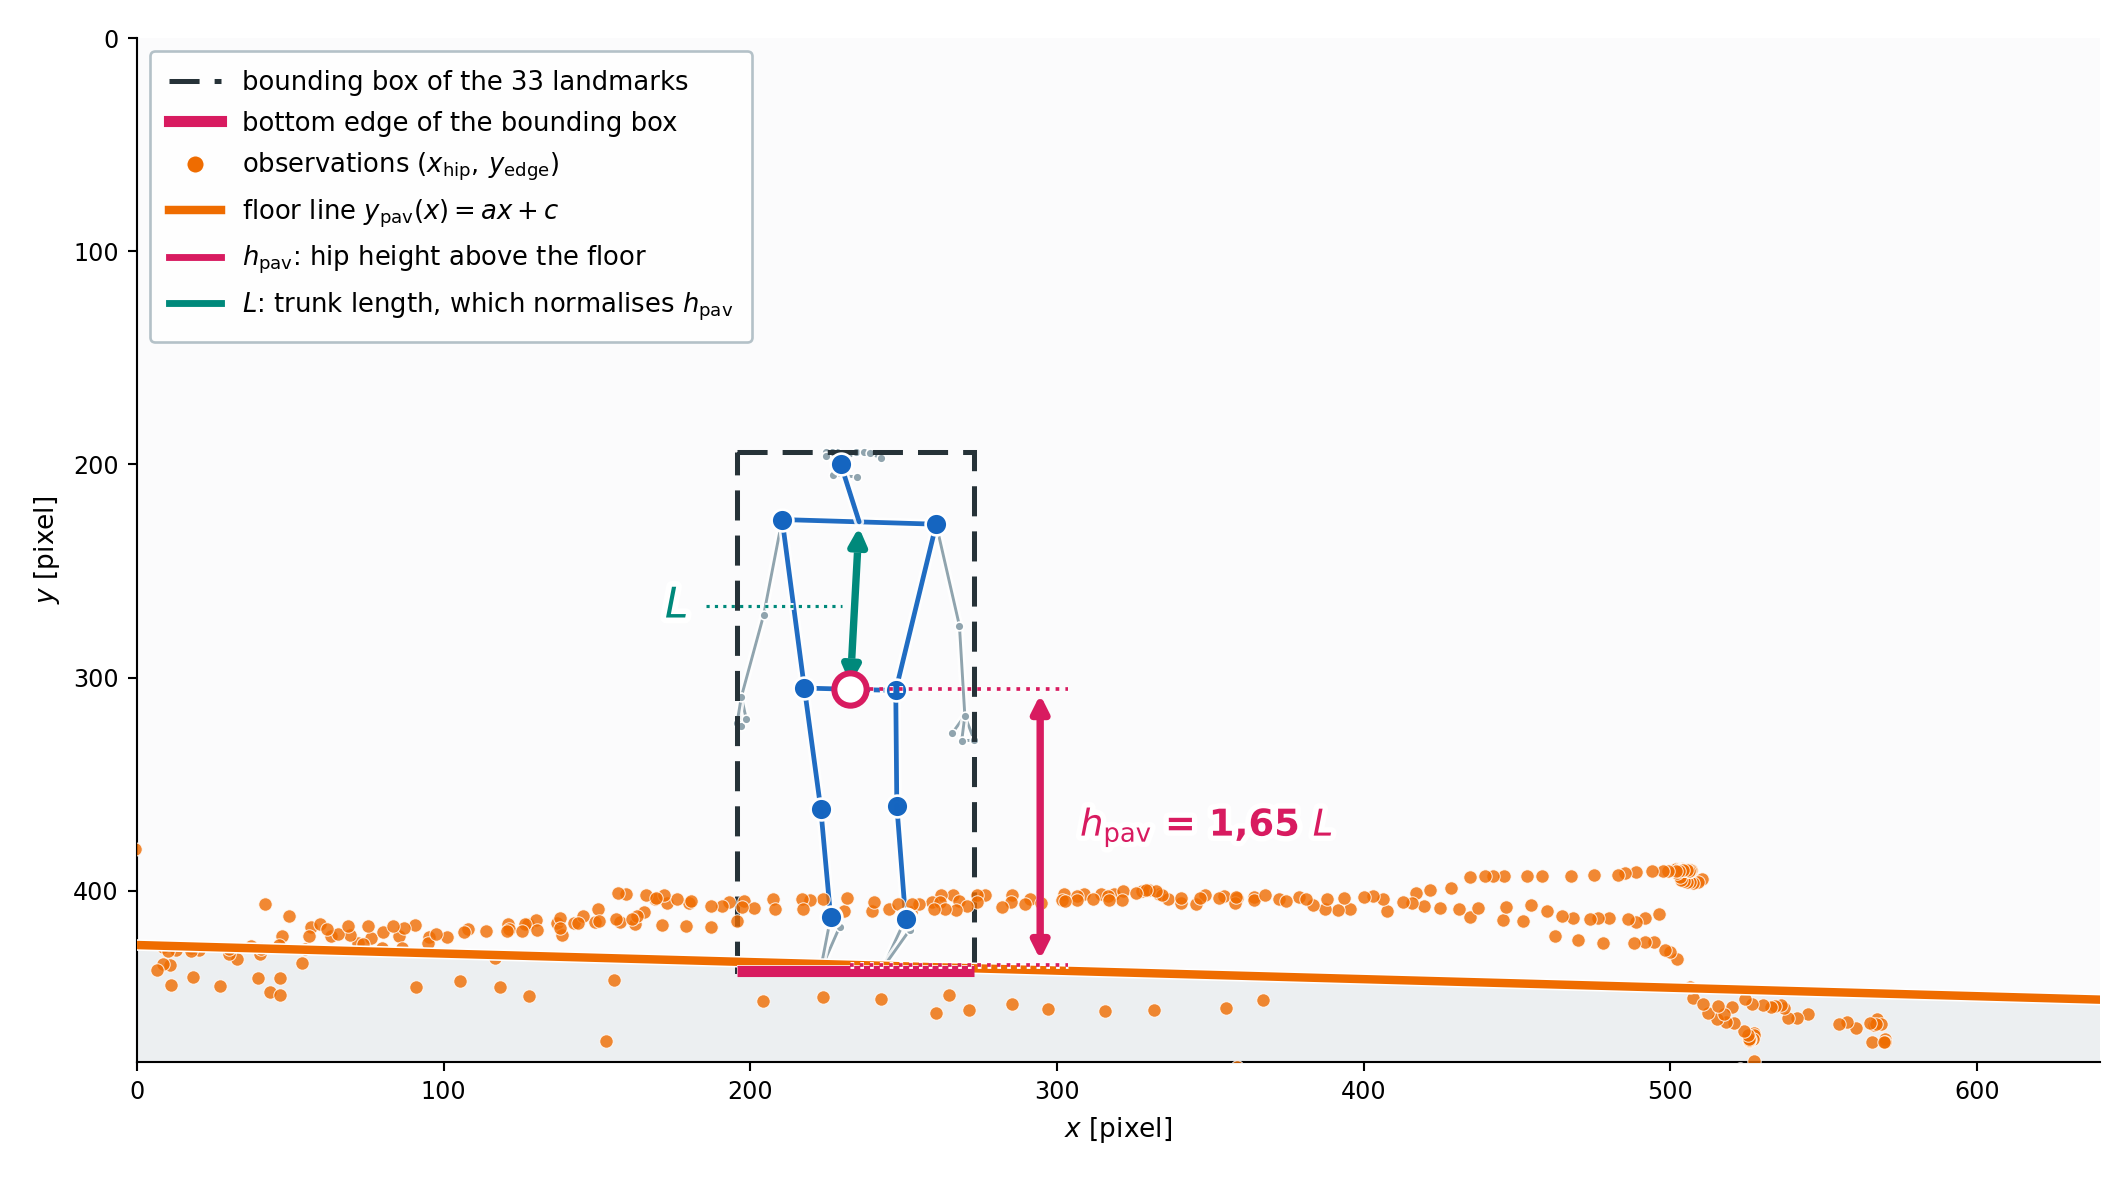
\includegraphics[width=\textwidth]{figure/fig_pavimento_en.png}
\caption{Estimating the height of the hips above the floor. From the frames
in which the person is standing, the points
\((x_{\text{bacino}}, y_{\text{bordo}})\) are collected and used to estimate the
floor line \(y_{\text{pav}}(x)\). The height \(h_{\text{pav}}\) is then computed
as the vertical distance between the centre of the hips and the floor line,
normalised with respect to the length of the trunk.}
\label{fig:pavimento}
\end{figure}

Dividing by \(L_{\text{tronco}}\) makes the quantity dimensionless and reduces the effect of the scale at which the person appears in the image. The parameters \(a\) and \(c\) remain instead tied to the individual installation, because they describe the position of the floor as observed from that camera.

The estimate uses the lower edge of the box containing all 33 landmarks, and some of them may be estimated outside the image when part of the body is not fully visible. The phenomenon concerns the extremities above all: in the frames examined, the tip of the foot is estimated below the lower edge in 48\% of cases and the wrist in 32\%.
In one recording used to check the effect on the estimate, 17,8\% of the observations exceed the lower limit of the image, with a median excess of 60 pixels over a height of 480. Repeating the computation after clipping the vertical coordinates to the height of the image, the estimated line shifts by 12 pixels, about one sixth of the length of the trunk in the sequence considered. Fitting over several observations reduces the effect of individual outliers, but does not remove it altogether, and it must be declared as a downward bias of the estimate.

The viewpoint of the camera also affects the measurement. For \(h_{\text{pav}}\) to be informative, the vertical displacement of the person must produce a visible variation in the image plane. A lateral view, placed roughly at chest height, meets this condition better than a strongly raised view. The dependence was verified by computing \(h_{\text{pav}}\) separately for the two cameras of the dataset and comparing, for each view, the distributions obtained in the fall frames and in the frames of daily activity. The results are reported in Section~\ref{sec:viewpoint}.

Finally, the floor line requires a certain number of observations of the person in an upright position. At system start-up the reference is therefore not immediately available and, until enough samples have been collected, \(h_{\text{pav}}\) cannot be used. The effect of this initial phase is verified on the domestic recordings in Chapter~\ref{cap:edge}.
One possible alternative would be to calibrate the floor once during installation and store \(a\) and \(c\) together with the configuration of the camera. This solution would avoid rebuilding the reference at every new run, but it was not implemented in the system developed, because a stored line remains valid only as long as the camera is not moved, whereas the online estimate adapts by itself.

In what follows, A3 denotes the basic body-centric representation, A3h the same representation with the addition of the height of the hips above the floor, and A3i the extension with the three integral quantities. The two extensions are independent and can also be used together.
With the addition of the height above the floor, the overall number of candidate features goes from 32 to \textbf{33}.

\section{Selecting the quantities by means of \emph{Dynamic Time Warping}}
\label{sec:dtw}

The 33 candidate features are not necessarily all useful for distinguishing a fall from daily activities. Before training, a preselection was therefore carried out by directly comparing the time series produced by the different features.

For this purpose \emph{Dynamic Time Warping} (DTW) was used, a technique which, unlike a distance computed point by point such as the Euclidean one, makes it possible to deform the time axis locally so as to align curves that describe similar shapes even when they evolve at different speeds, and which seeks the alignment producing the lowest overall cost. Two curves with a similar shape can thus turn out to be close even when the same change does not occur at the same instant.

In the present work the DTW is not used by the classifier, but only as an analysis tool to assess the separability of the features. The idea is that a useful quantity should produce similar trajectories among examples of the same class and, at the same time, different ones between falls and daily activities.
\begin{figure}[htbp]
    \centering
    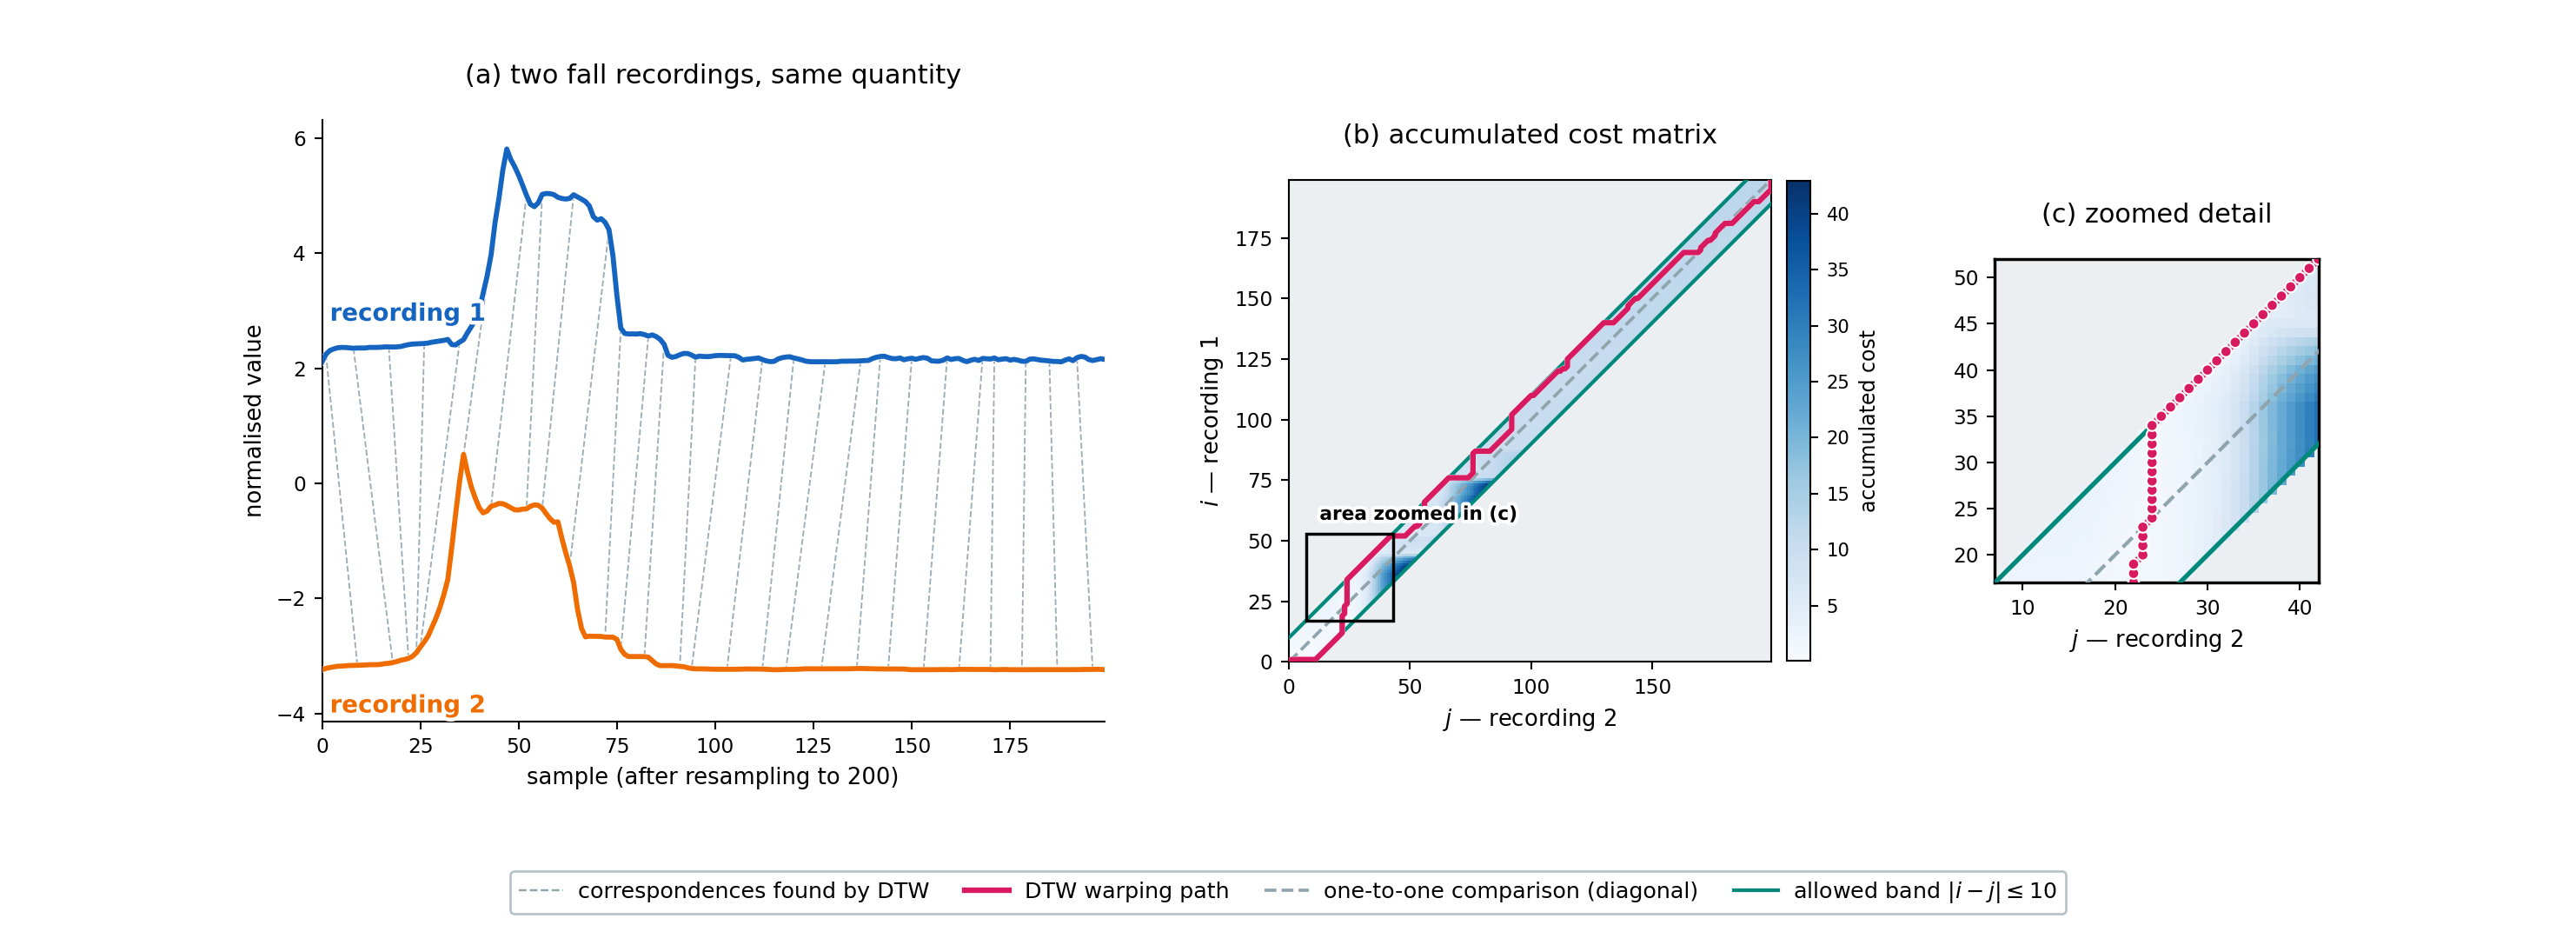
\includegraphics[width=\linewidth]{figure/fig_dtw_spiegazione_en.png}
    \caption{Example of alignment by DTW and of the band constraint used in the selection procedure.}
    \label{fig:dtw_allineamento}
\end{figure}

\subsection{Normalisation and resampling}

Before the comparison, every time series is normalised separately to zero mean and unit standard deviation:
\[
\tilde{x}_t = \frac{x_t-\mu_x}{\sigma_x}.
\]
This choice makes it possible to compare features with different scales and units of measurement: some are angles, others velocities, others still dimensionless ratios. Without this operation the distance would also be influenced by the numerical magnitude of the quantity, whereas at this stage what matters above all is the shape of the curve.

The fall recordings and those relating to daily activities have very different durations, about 180 and 820 frames respectively. Comparing such different sequences directly would require a very wide alignment band precisely in the comparison between the two classes.
In order to preserve the same meaning for the alignment constraint, after normalisation all the curves are resampled to a common length of 200 samples. This operation is used only in the DTW analysis and does not alter the data subsequently supplied to the classifier.

\subsection{Separability score and selection}

The temporal deformation allowed by the DTW is limited by imposing
\[
|i-j|\leq 10,
\]
where $i$ and $j$ are the indices of the samples in the two sequences. Small temporal shifts are thus admitted, while at the same time parts of the two curves that are too far apart are prevented from being matched. For each quantity three families of distances are computed:
\begin{itemize}
\item \(D_{FF}\), between pairs of fall recordings;
\item \(D_{AA}\), between pairs of daily activities;
\item \(D_{FA}\), between a fall and a daily activity.
\end{itemize}

A discriminative quantity should produce small distances within the same class and larger ones between the two classes. Denoting by
\[
\mu_{\mathrm{intra}}=\frac{\mu_{FF}+\mu_{AA}}{2},
\]
the mean intra-class distance, the separability score is defined as
\[
S=
\frac{\mu_{FA}}
     {\mu_{\mathrm{intra}}+\varepsilon},
\]
where \(\varepsilon\) prevents division by zero. A value close to one indicates that the inter-class distances are similar to the intra-class one, while larger values indicate a sharper difference.

UP-Fall observes the same events from two different viewpoints. The initial analysis computed a single score, considering the recordings of the two cameras together. That choice may, however, favour a feature that is highly discriminative in one view and poorly informative in the other. The score is therefore computed separately for each view, and for the selection
\[
S_{\text{robusto}} = \min\big(S_{\text{cam}_1},\ S_{\text{cam}_2}\big).
\]
is considered.

The lower value is chosen, rather than the mean, so as to prevent a feature that is effective from one view alone from nonetheless obtaining a high score. The effect of the viewpoint on the values obtained is analysed in Section~\ref{sec:viewpoint}.

The DTW, however, assesses every feature separately, and two quantities may both obtain a good score while describing almost the same information. In order to limit this redundancy, the features are ordered according to \(S_{\text{robusto}}\) and considered in sequence. A new quantity is retained only if its absolute correlation with all those already selected satisfies
\[
|\rho|<0{,}85.
\]

The correlation is computed only on the frames with a valid pose, so that the values inserted where the pose is missing do not create correlations that have nothing to do with the content of the features.
Four features are excluded from the subset for precisely this reason, and are reported in Table~\ref{tab:ridondanti}.

\begin{table}[ht]
\centering
\caption{Quantities excluded for redundancy, with the feature already selected with respect to which the correlation threshold is exceeded.}
\label{tab:ridondanti}
\begin{tabular}{@{}llc@{}}
\toprule
\textbf{Excluded} & \textbf{Redundant with} & \textbf{\(|\rho|\)} \\
\midrule
\texttt{A2\_angolo\_tronco}    & \texttt{A2\_testa\_rel\_y}    & 0,97 \\
\texttt{A3\_testa\_rel\_y}     & \texttt{A2\_testa\_rel\_y}    & 0,98 \\
\texttt{A2\_escursione}        & \texttt{A3\_escursione}       & 0,86 \\
\texttt{A3\_ginocchia\_rel\_y} & \texttt{A3\_caviglie\_rel\_y} & 0,93 \\
\bottomrule
\end{tabular}
\end{table}

The procedure leads to the selection of 12 of the 33 candidate quantities. In decreasing order of $S_{\mathrm{robusto}}$, the features selected are
\texttt{A2\_testa\_rel\_y}, \texttt{A2\_discesa},
\texttt{A2\_percorso}, \texttt{A1\_discesa}, \texttt{A3\_discesa},
\texttt{A3\_escursione}, \texttt{A3\_caviglie\_rel\_y}, \texttt{A3\_percorso},
\texttt{A3\_hip\_vel}, \texttt{A3\_testa\_vel\_rel}, \texttt{A1\_percorso} and
\texttt{A1\_escursione}.

The mean correlation among them is \(0{,}435\). The subset comprises features coming from all three representations, and eight of the twelve are integral quantities. A particular case is that of the height of the hips above the floor. The feature obtains \(1{,}541\) on the lateral view, the second highest score among the 33, and \(1{,}124\) on the raised one. The gap, \(0{,}417\), is the largest of the whole set.

The minimum between the two views therefore places it twenty-first, and the selection excludes it. The result is consistent with the aim of the criterion: to prevent quantities whose effectiveness depends heavily on the position of the camera from being favoured. The acquisition protocol envisaged for the installed system does, however, use a lateral view, in which the height above the floor shows its most favourable behaviour. For this reason a second configuration is also analysed, denoted by \textbf{DTWH}, obtained by adding the height of the hips above the floor to the 12 features selected by DTW.

\begin{table}[htbp]
\centering
\caption{Abbreviations used to denote the main feature configurations.}
\label{tab:sigle}
\begin{tabular}{@{}llc@{}}
\toprule
\textbf{Abbreviation} & \textbf{What it contains} & \textbf{No.} \\
\midrule
A1, A2, A3 & the set of the three representations, integral quantities included & 32 \\
A3base & basic A3 representation & 9 \\
A3h & A3 with the height of the hips above the floor & 10 \\
A3i & A3 with the three integral quantities & 12 \\
\textbf{DTW} & \textbf{subset obtained from the automatic selection} & \textbf{12} \\
DTWH & DTW plus the height above the floor & 13 \\
\bottomrule
\end{tabular}
\end{table}

One last point concerns the relationship between this selection and the \emph{leave-one-subject-out} protocol. In a LOSO evaluation, the subject used as test should take part in no operation that derives information from the data, feature selection included. In the pipeline used, the DTW selection was instead carried out once over the whole dataset before the LOSO, and the same 12 features were subsequently used in every fold. The subject left out therefore contributed indirectly to the choice of the features. This introduces a form of \emph{data leakage} that must be borne in mind when reading the results.

In order to quantify its effect, in Chapter~\ref{cap:sperimentale} the procedure is repeated separately for each fold, excluding the test subject every time and comparing the subset obtained with the one adopted. The normalisation described at the beginning of this section is the one internal to the DTW analysis, and is applied separately to the individual curves. It is not to be confused with the normalisation of the data supplied to the classifiers, which is instead estimated within each fold on the training data alone, as described in Section~\ref{sec:classificatori}.

\section{Construction of the temporal windows}
\label{sec:finestre}

The classifier receives as input sequences of features organised into temporal windows. The same body configuration may appear in different activities, whereas the way the pose changes over time supplies the information that distinguishes a fall from an ordinary daily activity.
Denoting by $f_t$ the feature vector at sample $t$, a window of length \(L\) is defined as
\[
X_t = [\,f_t, f_{t+1},\dots, f_{t+L-1}\,].
\]

Before the windows are built, the sequence extracted at about 18 fps is subsampled by taking one sample in two, so that the classifier works at a nominal frequency of about 9 samples per second. In the configuration used, a length $L=22$ is chosen which, at that frequency, corresponds to about
\[
\frac{22}{9}\simeq 2{,}44\text{ s}.
\]

The choice of length is a compromise. A window that is too short observes only part of the movement and may not contain enough context to distinguish a fall from a rapid activity; a very long window includes more frames that do not belong to the phase of interest and increases the time needed for a sequence to be complete.

The value of 22 samples was inherited from an earlier configuration that used 45 samples at 18 fps, thus preserving a similar duration. Windows of 28, 36 and 44 samples were also considered, corresponding to intervals between about $2{,}4$ and $4{,}9$ s. The laboratory $F_2$ improves systematically as the length increases, but in the final configuration $L=22$ was retained in order to limit latency. The comparison between the different lengths is reported in Chapter~\ref{cap:sperimentale}. The windows are built with a stride of two samples: two consecutive windows therefore share 20 samples out of 22 and are strongly overlapping. This choice reduces the risk that a fall falls across two windows without being sufficiently represented in either. Neighbouring windows cannot, however, be considered independent observations, an aspect that is taken into account when separating training data from test data.

Subsampling and the stride of the window denote two different operations. The first establishes which samples enter the classifier; the second establishes how often a new window is built. The features are computed before subsampling: a dynamic quantity contained in a sample therefore retains the value obtained during extraction on the original sequence, and subsampling comes into play only in the subsequent construction of the windows. Finally, a window is built only within a continuous stretch with a valid pose. If the estimator loses the person, the sequence is interrupted and construction resumes only when a sufficient number of consecutive frames is available again. In this way a window never contains frames belonging to two intervals separated by a loss of tracking.

\section{Definition of the task and assignment of the label}
\label{sec:compito}

A fall comprises two distinct moments: the movement by which the person loses their balance and reaches the ground, and the subsequent state in which they remain on the ground. The UP-Fall recordings were observed and annotated manually at frame level, distinguishing three phases:
\begin{itemize}
    \item \textbf{ordinary activity}, corresponding to the phase preceding the loss of balance;
    \item \textbf{transition}, from the loss of balance until arrival on the ground;
    \item \textbf{post-fall state}, in which the person remains on the ground.
\end{itemize}

The labels $0$, $1$ and $2$ were associated with the three conditions respectively. These annotations constitute the frame-level reference from which the labels of the temporal windows are derived. The three phases have different durations. Considering the 50 fall recordings of Camera~1, relating to the ten subjects used, the values reported in Table~\ref{tab:durate_fasi} are obtained.

\begin{table}[ht]
\centering
\caption{Duration of the three phases in the UP-Fall fall recordings considered for Camera~1.}
\label{tab:durate_fasi}
\begin{tabular}{lccc}
\hline
\textbf{Phase} & \textbf{Median} & \textbf{10\% decile} & \textbf{90\% decile} \\
\hline
Before the fall & 0,94 s & --- & --- \\
Transition & 3,11 s & 2,05 s & 3,94 s \\
Post-fall state & 5,97 s & 4,82 s & 6,89 s \\
\hline
\end{tabular}
\end{table}

The transition therefore lasts a little over three seconds, while the post-fall state occupies on average an even longer interval. Distinguishing the two phases separates the event of falling from the condition that follows it, and the distinction is not academic: from an applicative point of view, including the post-fall state as well would be the natural choice, since remaining on the ground is the condition that matters in monitoring and lasts far longer than the dynamic phase.

The problem emerges when one considers the daily activities that produce a similar final configuration. A person may find themselves in a horizontal position without having fallen, and UP-Fall contains the activity \emph{laying}, in which the subject lies down voluntarily: it comprises 20.980 frames, about 18\% of the dataset, labelled as daily activity, against 10.524 belonging to the post-fall state.
For this reason the two phases are kept separate in the reference ground truth. In the final configuration of the system the transition is used as the main positive event, while the post-fall state is kept distinct, both in order to build the window labels correctly and in order to compare different formulations of the problem.

Once the three phases have been defined at frame level, it is necessary to establish how to transfer these annotations to the temporal windows. A window may comprise samples belonging to different phases and cannot therefore be labelled on the basis of a single frame.

For the construction of the main labels it was decided to take into account the temporal arrangement of the frames within the window as well. A simple total count assigns the same weight to samples spread along the whole sequence and to samples concentrated in the same interval. For this reason a $K$-of-$M$ criterion was adopted. Denoting by $m_t$ a binary variable equal to one when the frame belongs to the phase considered,
\[
\max_i \sum_{t=i}^{i+M-1} m_t \geq K.
\]
The phase is considered present when at least $K$ frames associated with it lie within a local interval of $M$ samples.
For the transition $K=5, \qquad M=8$ are used, while for the post-fall state $K = 10, \qquad M = 15$. These values form part of the preprocessing procedure and were not obtained by directly optimising the performance of the classifier.

Starting from the presence of the transition and of the post-fall state, three formulations for training were considered:
\begin{itemize}
\item \textbf{discard}: the transition constitutes the positive class, while the windows belonging exclusively to the post-fall state are excluded from training;
\item \textbf{fall}: transition and post-fall state are both considered positive;
\item \textbf{three classes}: ordinary activity, transition and post-fall state are kept as separate classes. \end{itemize}

The three formulations therefore use the labels (0), (1) and (2) defined at frame level and the (K)-of-(M) criterion described above. In order to keep the same verification set, two labels are associated with every window. The first, $y_{\text{train}}$, depends on the formulation used during training. In the \textbf{discard} mode, the windows belonging exclusively to the post-fall state are kept in the dataset but marked with
\[
y_{\text{train}}=-1,
\]
and therefore take no part in training.

The second label, denoted by $y_{\text{allarme}}$, is instead used for the common evaluation and equals one when the transition or the post-fall state is present in the window. In this way the different formulations can be evaluated on the same set of windows.

As additional information, the annotations of \emph{OmniFall}~\cite{SN} were also used, which reannotates several fall detection datasets, among them UP-Fall, distinguishing in particular:
\begin{itemize}
    \item \texttt{fall}, relating to the fall event;
    \item \texttt{fallen}, relating to the state following the fall;
    \item \texttt{lie\_down}, relating to lying down intentionally;
    \item \texttt{lying}, relating to the subsequent lying position.
\end{itemize}

These annotations were not used to build the labels (0), (1) and (2). They were added afterwards to the features already extracted, converting the time intervals of OmniFall into the corresponding frame intervals at the nominal frequency of 18 fps. By this procedure it was possible to associate an OmniFall label with 98,5\% of the frames.

The three formulations just described must, however, be distinguished from the three tasks \emph{event}, \emph{state} and \emph{alarm} analysed in Chapter~\ref{cap:sperimentale}, because those of the present chapter use the labels (0/1/2) and the local (K)-of-(M) criterion, whereas the three tasks of the experimental chapter are built on the OmniFall classes and consider a class present when at least five of its frames appear in the window, irrespective of their temporal arrangement. The correspondence between the two sets is therefore only partial. \emph{Event} treats as positive the same phase as the \textbf{discard} mode, but treats windows of post-fall state alone as negative instead of excluding them from training. \emph{Alarm} coincides instead with \textbf{fall} in the definition of the positive class. The task \emph{state} has no counterpart among the three formulations of the present chapter, while the formulation \textbf{three classes} has no counterpart among the three tasks based on OmniFall.

\section{Classifiers and training}
\label{sec:classificatori}

The preceding sections lead from the frame to a window made of 22 samples and 12 features. It remains to be established how to use this sequence in the three training formulations defined in Section~\ref{sec:compito}.
Six architectures are compared in this work: Random Forest, LSTM, GRU, 1D CNN, Transformer and a graph network. The choice comprises models that are very different from one another, but the comparison is built so as to keep the other elements of the pipeline unchanged. The architectures therefore use the same representation, the same LOSO folds and the same decision rule.

The comparison is not meant to establish which family is the best in absolute terms. From one study to another, besides the classifier, the dataset, features, preprocessing, data split and decision threshold usually change as well, and a difference in performance may depend on any one of these. Keeping them fixed allows the differences observed to be attributed to the architecture of the classifier. For LSTM, GRU, 1D CNN, Transformer and the graph network the input keeps the shape $22 \times 12$, where the 22 rows correspond to the samples of the temporal window and the 12 columns to the selected features.

The Random Forest is instead used as a non-sequential reference, and serves to verify how much the architecture really weighs at fixed representation: if a model that does not follow the temporal order obtains results similar to those of a recurrent network, the advantage of modelling the sequence explicitly is limited under the conditions considered.
For each of the 12 features, mean, standard deviation, minimum, maximum, first and last sample are computed, producing $12\times6=72$ values. The first and last sample are there because without them the summary would preserve no direction, and a fall and a getting-up would turn out identical.
The configurations used are reported in Table~\ref{tab:modelli}.

\begin{table}[htbp]
\centering
\caption{Architectures used and their complexity. For the Random Forest
the value reported is the overall number of nodes of the trees, which is not a
parameter learnt by gradient descent but is what determines its
occupation in memory.}
\label{tab:modelli}
\begin{tabular}{@{}p{2.2cm}p{8.8cm}r@{}}
\toprule
\textbf{Model} & \textbf{Architecture} & \textbf{Parameters} \\
\midrule
GRU & two recurrent layers of 64 and 32 units, with dropout of 0,3 & 24.483 \\
LSTM & two recurrent layers of 64 and 32 units, with dropout of 0,3 & 32.227 \\
1D CNN & two temporal convolutional blocks with 64 and 128 filters, kernel of size 5, batch normalisation, subsampling by a factor of 2 and dropout of 0,3; final global average pooling & 46.147 \\
Transformer & projection to 64 dimensions, learnt positional encoding, one self-attention block with 4 heads, feed-forward layer of 128 units and global average pooling & 34.499 \\
GNN & two spatio-temporal blocks with learnt adjacency among 12 nodes, \(1\times1\) convolution with 32 channels, temporal convolution with kernel 5 and batch normalisation & 12.323 \\
Random Forest & 50 trees with no preset depth limit, trained on the 72 values derived from each window & 12.928 nodes \\
\bottomrule
\end{tabular}
\end{table}

GRU and LSTM have the same general structure and differ only in the type of recurrent cell. For the same number of units, the GRU uses fewer parameters. The 1D CNN instead processes the window by means of convolutions along the temporal dimension, while the Transformer uses a self-attention mechanism with positional encoding.

In the graph network, in order to keep the representation consistent with that of the other classifiers, the nodes are not the anatomical joints but the twelve input features, and the relations among them are learnt during training. The results of the GNN therefore refer to this configuration and do not constitute a general assessment of graph networks applied directly to the human skeleton.

The same training protocol, reported in Table~\ref{tab:addestramento}, is used for the five neural networks.

\begin{table}[htbp]
\centering
\caption{Protocol used for training the neural networks.}
\label{tab:addestramento}
\begin{tabular}{@{}p{4.6cm}p{9.0cm}@{}}
\toprule
\textbf{Element} & \textbf{Value} \\
\midrule
Input & \(22\times12\): 22 samples and 12 features \\
Output & distribution over 2 or 3 classes, according to the training formulation \\
Loss function & categorical cross-entropy \\
Class weights & inversely proportional to the frequency of the classes \\
Optimiser & Adam, initial learning rate \(10^{-3}\) \\
Epochs & at most 40 \\
Batch size & 16 \\
Early stopping & area under the curve of the \emph{alarm probability} on the validation set, patience of 8 epochs and restoration of the best weights \\
Learning-rate reduction & factor \(0{,}5\) after 4 epochs without improvement, down to a minimum of \(10^{-5}\) \\
Random seed & 42 \\
Repetitions & one per fold \\
\bottomrule
\end{tabular}
\end{table}

The decision threshold is kept fixed at
\[
\tau = 0{,}50,
\]
for all the architectures and for all the folds. The networks always produce a \emph{softmax} distribution, even in the binary case. In this way the alarm probability is derived in the same way for all the training formulations. In the binary case two classes are considered, whereas in the three-class formulation ordinary activity, transition and post-fall state are kept separate.

The Random Forest does not use the training procedure of Table~\ref{tab:addestramento}. The model is trained once for each fold using 50 trees and unlimited depth.
The hyperparameters of the models reported in Tables~\ref{tab:modelli} and~\ref{tab:addestramento} were not optimised separately on the test folds. The random seed is fixed at 42 before each model is built, and every architecture is trained only once per fold. Consequently, the dispersion reported in the results measures the variability among the subjects left out in the different LOSO folds, and not the variability due to different initialisations of the same model.

One last point concerns the operations that derive information from the data. In a LOSO protocol the subject used for the test should contribute to none of these operations.
The normalisation supplied to the classifiers is estimated within each fold using only the training data, and is then applied unchanged to the validation and test data. The threshold and the hyperparameters of the models do not depend on the test subject either, because they are kept fixed.

As discussed in Section~\ref{sec:dtw}, feature selection by DTW was applied once to the whole dataset before the LOSO, and the same 12 features were then used in every fold. The value \(K=31\) of the integral quantities was likewise chosen after a check that involved data subsequently used in the evaluation. Both aspects are therefore regarded as limitations of the protocol.

In order to assess their effect, the two procedures were repeated excluding the test subject each time. The checks, reported in Chapter~\ref{cap:sperimentale}, are however different: in the case of the DTW, the features selected within each fold are compared with those adopted in the main configuration, whereas for (K) the performance obtained is compared directly. In this second case the check moreover shows that the initial choice of (K=31) did not increase performance with respect to the selection carried out within the individual folds.

\section{From classifier output to alarm event}
\label{sec:allarme}

The classifier produces one decision per window, whereas the installed system must generate alarm events. The two things do not coincide: the windows are strongly overlapping, and a single fall may therefore produce several consecutive positive predictions.

In order to use the same rule across the different formulations of the problem, an alarm score was defined from the output of the classifier. In the binary case it coincides with the probability of the positive class; in the three-class case it corresponds to the overall probability of not belonging to the normal class, that is
\[ p_{\mathrm{allarme}} = 1-p_{\mathrm{normale}}. \]
A window is considered positive when
\[ p_{\mathrm{allarme}} \geq 0{,}50. \]

A single positive window does not, however, produce an alarm. The alert is generated only when five consecutive windows turn out positive. If a window drops below the threshold before that number is reached, the count is reset. The condition can therefore be written as a persistence of five consecutive positive decisions.

The alarm is raised at the moment the fifth consecutive positive window is observed. The four preceding windows are needed in order to verify the persistence and cannot therefore be taken as the instant at which the system has already recognised the event. After an alarm has been raised, a refractory interval of $30\text{ s}$ is applied. During this interval no new alerts can be generated. The 30 seconds are counted from the last alarm raised. If the positive condition continues beyond the end of the refractory interval, the system can therefore generate a new alert.

The configuration adopted can be summarised as follows: \begin{table}[htbp]
\centering
\caption{Rule used to turn the predictions on the windows into
alarm events.}
\label{tab:allarme}
\begin{tabular}{@{}p{4.5cm}p{8.5cm}@{}}
\toprule
\textbf{Element} & \textbf{Value} \\
\midrule
Threshold & \(p_{\mathrm{allarme}}\geq0{,}50\) \\
Persistence & 5 consecutive positive windows \\
Reset & at the first window below threshold \\
Instant of the alarm & fifth consecutive positive window \\
Merging of events & the subsequent positive windows belong to the same alert for as long as the refractory interval lasts \\
Refractory interval & 30 s from the last alarm raised \\
End of the event & not defined: the alert is an instant, not an interval \\
\bottomrule
\end{tabular}
\end{table}

The system emits instants of alarm and computes no closure of the event: what the parameters delimit is the frequency with which the alerts may repeat, not the duration of an alert.
A very long sequence of positive predictions does not necessarily correspond to a single alarm. In real recordings some false positives may last a long time, for example when a person remains lying on the sofa. If the score stays above the threshold for more than 30 seconds, the system may generate a new alarm when the refractory interval ends. The number of alerts therefore depends also on the duration chosen for this interval, and not only on the predictions of the classifier.

This transformation also distinguishes two levels of evaluation. The metrics computed on the individual windows describe the behaviour of the classifier, whereas the number of alarms produced per unit of time describes the behaviour of the installed system. The two quantities are not directly equivalent: many consecutive positive windows may produce a single alert, whereas isolated positive predictions may produce no alarm at all. Chapter~\ref{cap:edge} analyses their effect during real operation and also compares alternative rules, among them \(m\)-of-\(n\) criteria, accumulation of the score and hysteresis with two thresholds.

